% File: VTthesis_template.tex
% Created: Thu Mar 24 11:00 AM 2016 EDT
% Last Change: Thursday, December 19, 2019
% Author: Alan M. Lattimer, VT
% With modifications by Carrie Cross, Robert Browder, and LianTze Lim. 
% 
% This template is designed to operate with XeLaTeX.
% 
% All elements in the Title, Abstract, and Keywords MUST be formatted as text and NOT as math.
% 
% Further instructions for using this template are embedded in the document. Additionally, there are comments at the end of the file that give suggestions on writing your thesis.  
% 
% In addition to the standard formatting options, the following options are defined for the VTthesis class: proposal, prelim, doublespace, draft. 

\documentclass[doublespace,draft,nopageskip]{VTthesis} % nopageskip - Removes arbitrary blank pages.

% Using the following header instead will create a draft copy of your thesis
% \documentclass[doublespace,draft]{VTthesis}

% The lipsum package is just included to put dummy text in the document in order to demonstrate page headers and table of contents behavior. You should remove it once you begin writing your actual thesis or dissertation.
\usepackage{lipsum}

\usepackage{threeparttable}


% Title of your thesis
\title{Title of your thesis goes here}

% You should include 3-5 keywords, separated by commas
\keywords{Some Keywords, Subject matter, etc.}

% Your name, including middle initial(s)
\author{Deheng Song}

% Change this to your program, e.g. Physics, Civil Engineering, etc.
\program{Physics} 

% Change this to your degree, e.g. Master of Science, Master of Art, etc.
\degree{Doctor of Philosophy} 

% This should be your defense date:
\submitdate{Dec 17, 2021} 

% Committee members. Only have five readers and one chair available.
% Only use the ones you need and don't include the ones you don't need.
% You can also declare a Co-advisor. If you do, the principal and co-advisors
% will be listed as co-advisors on the title page.  Per the VT ETD standards, 
% you should not include titles or educational qualifications such as PhD or Dr.
% You should, however, include middle initials if possible.
\principaladvisor{Shunsaku Horiuchi}
% \coadvisor{Vicente Esparza}
\firstreader{Giti}
\secondreader{John}
\thirdreader{Tatsu}
% \fourthreader{Fourth Committee Member}
% \fifthreader{Fifth Committee Member}

% The dedication and acknowledgement pages are optional. Comment them out to remove them.
% \dedication{This is where you put your dedications.}
\acknowledge{This is where you put your acknowledgments.}

% The abstract is required.
\abstract{Give a brief description of your thesis here.}
% \abstract{\lipsum [1-4]}

% The general audience abstract is required. There are currently no word limits.
\abstractgenaud{You are also required as of Spring 2016 to include a general audience abstract. This should be geared towards individuals outside of your field that may be reading seeking information about your work. You should avoid language that is particular to your field and clearly define any terms that may have special meaning in your discipline.}

\begin{document}
% The following lines set up the front matter of your thesis or dissertation and are required to ensure proper formatting per the VT ETD standards. 
\frontmatter
\maketitle
\tableofcontents

% The list of figures and tables are now optional per the official ETD standards.  Unless you have a very good reason for removing them, you should leave these lists in the document. Comment them out to remove them.
\listoffigures
\listoftables
% \printnomenclature %Creates a list of abbreviations. Comment out to remove it. 

% % sample text for abbreviations:
% NLP is a field of computer science, artificial intelligence, and linguistics concerned with the interactions between computers and human (natural) languages.

% \nomenclature{NLP}{Natural Language Processing}

% $\sigma$ is the eighteenth letter of the Greek alphabet, and carries the 's' sound. In the system of Greek numerals, it has a value of 200. 

% \nomenclature{$\sigma$}{The total mass of angels per unit area}

% The following sets up the document for the main part of the thesis or dissertation. Do not comment out or remove this line.
\mainmatter

% now go ahead and start writing your thesis
\chapter{Introduction} \label{ch:introduction}
\lipsum[1]

% Copy/paste the code below to add sections and subsections to each chapter. Add your own text to the chapter and (sub)section labels to create custom headings.          
\section{One Section} \label{se:one_section}
\lipsum[2]
\subsection{A sub-section} \label{ss:this_subsection}
\lipsum[1-4]
\section{Another Section} \label{se:another_section}
\lipsum[1-2]

\chapter{Inverse Compton emission from millisecond pulsars in the Galactic bulge} \label{ch:IC_MSPs}

\section{Introduction}
In the past decade, the Fermi Large Area Telescope (Fermi-LAT) has provided accurate observations of the gamma-ray sky, of which the Galactic center (GC) remains one of the most intriguing and intricate regions. It is of paramount importance to map the gamma-ray emissions from the GC to better understand the properties of cosmic rays (CRs), the interstellar medium (ISM), and tests of dark matter (DM) in the inner regions of our Galaxy. Using template fitting techniques to regress out the Galactic and extragalactic diffuse emissions, multiple studies~\cite{Goodenough:2009gk,Vitale:2009hr,Hooper:2010mq,Abazajian:2012pn,Gordon:2013vta, Macias:2013vya,Hooper:2013rwa,Abazajian:2014fta,Daylan:2014rsa,Calore:2014xka,Zhou:2014lva,TheFermi-LAT:2015kwa,TheFermi-LAT:2017vmf} have found an excess of gamma rays towards the GC extending up to $\sim\pm$20 degrees in latitude. Often referred to as the Galactic center excess (GCE), this excess emission has a centrally peaked spatial morphology that is roughly spherically symmetric with a radial power law of slope $\sim$2.4, and a curved energy spectrum peaking at $\sim$3 GeV. Some authors have argued that the GCE is consistent with a DM emission~\cite{Goodenough:2009gk,Abazajian:2012pn,Gordon:2013vta,Macias:2013vya,Calore:2014xka,Daylan:2014rsa} given its similarities to simplified predictions of weakly interacting massive particle DM models.

However, studies have also shown that the origin of the GCE can be explained by astrophysical sources, such as a population of unresolved gamma-ray-emitting millisecond pulsars (MPSs)~\cite{Abazajian:2010zy,Abazajian:2012pn,Gordon:2013vta,Macias:2013vya,Calore:2014xka,Daylan:2014rsa}. While there is ongoing debate regarding the consistency of the GCE with the luminosity function of MSPs measured elsewhere in the Galaxy\cite{Cholis:2014lta, Hooper:2015jlu, Ploeg:2017vai, Bartels:2018xom}, evidence supporting the MSP hypothesis is mounting. For example, population synthesis simulations~\cite{Gonthier:2018ymi} show that $\sim$$10^4$ MSPs can inhabit the GC region and explain the GCE. Also, subthreshold photon-count statistics have shown detectable features that can be used to distinguish between the MSPs and DM interpretations of the GCE. In particular, Refs.~\cite{Lee:2015fea,Mishra-Sharma:2016gis} introduced a new statistical technique called the non-Poissonian template fit which can be used for characterizing populations of unresolved point sources at fluxes below the detection threshold. They have shown that an unresolved population of point sources just below the sensitivity of the LAT is responsible for the GCE.

More recently, Refs.~\cite{Macias:2016nev, Bartels:2017vsx,  Macias:2019omb} investigated whether the spatial morphology of the GCE is better described by the distribution of stars or by DM. It has been firmly established that the bulk of the stars in the GC region form a so-called box/peanut-bulge structure~\cite{Dwek:1995xu,Freudenreich:1997bx,LopezCorredoira:1999dg,Nataf:2010wf,Wegg:2013upa}. The density distribution of these bulge stars can be reasonably described by a triaxial geometric function~\cite{Freudenreich:1997bx,Nataf:2010wf,Wegg:2013upa} extending in length to a few kpc from the GC. In addition to the box/peanut-bulge, there is a distinct stellar population in the innermost $\sim$200 pc of the Galaxy called the nuclear bulge (NB)~\cite{Nishiyama:2013eba}. Reference~\cite{Macias:2016nev} used two different stellar maps for the box/peanut-bulge~\cite{Freudenreich:1997bx,Ness:2016aaa} and also considered the NB of Ref.~\cite{Nishiyama:2013eba}, and demonstrated that such nonspherical bulge morphologies provide a significantly better fit to the GCE than a spherical Navarro-Frenk-White squared (NFW$^2$) spatial map describing a DM annihilation signal. Importantly, that article showed that once a bulge model is included in the analysis, there is no longer statistically significant evidence for a NFW$^2$ component. These results have been corroborated by Ref.\cite{Bartels:2017vsx} using a different and more flexible analysis method~\cite{Storm:2017arh} and by Ref.~\cite{Macias:2019omb} using an improved Galactic diffuse emission model.

The population of MSPs in the Galactic bulge would not only produce prompt gamma-ray emission correlated with their spatial distribution, but also inject $e^\pm$ into the interstellar environment. These CR $e^\pm$ can produce secondary emissions by interacting with the ISM and magnetic field. It has been pointed out that while the prompt gamma rays from MSPs are expected to follow the morphology of the source distribution, secondary emissions---inverse Compton (IC), bremsstrahlung, and synchrotron radiation---are expected to have different morphologies, since they also depend on their relevant targets, i.e., the interstellar radiation field (ISRF), the gas distribution, and the magnetic field of the Galaxy, respectively. The IC component is a result of an energy-dependent convolution of the spatial morphology of the CR $e^\pm$ sources with the ambient photon fields from starlight, infrared (IR) light, and the cosmic microwave background (CMB).

Previous works~\cite{Yuan:2014yda,Petrovic:2014xra} have studied the secondary IC emission at $\sim$GeV-TeV energies from MSP $e^\pm$ interacting with the ISRF assuming a \emph{spherically symmetric} distribution of MSPs. Under such an assumption, Ref.~\cite{Lacroix:2015wfx} searched for secondary gamma-ray emission from MSPs by performing template fits to the GCE data, and found it to be difficult to detect or constrain the putative secondary IC component from an unresolved population of MSPs using Fermi-LAT data alone. However, as discussed above, there is now growing evidence for a significant departure from spherical symmetry.

Nonspherical source morphologies have been explored on small ($<$1 kpc) scales. For example, in a region overlapping with the NB called the Galactic ridge, Ref.~\cite{Macias:2014sta} showed that several different CR scenarios can explain the multiwavelength data taken from this patch of the sky. In addition, Ref.~\cite{Carlson:2015ona} evaluated the impact of star-forming activity in the Galactic ridge on the GCE properties. The study by Ref.~\cite{Gaggero:2017jts} solved the diffusion equation for CRs with a position-dependent diffusion coefficient and explained the recent H.E.S.S.~\cite{Abramowski:2016mir} measurements from this region by the interaction of the CRs with the gas in the central molecular zone (CMZ). Reference~\cite{Guepin:2018jkb} explained the H.E.S.S. measurements by MSPs accelerating CR protons.

In this paper, we revisit the IC emission from MSP $e^\pm$ focusing on a potential \emph{nonspherical} source morphology related to the Galactic bulge structure. Reference~\cite{Abazajian:2014hsa} looked for and found a gamma-ray component following the IR distribution in the GC. The authors interpreted this as IC emission correlating with the distribution of optical light, but a propagation of the underlying $e^\pm$ was not performed. Here, we use the publicly available propagation code \texttt{GALPROP}\cite{Strong:1998fr,Galprop,Galpropsupplementary} and make detailed predictions for the spectrum and morphology of the IC emission at 100 MeV-100 TeV energies. For the spatial morphology of MSP $e^\pm$, we use a three-dimensional (3D) stellar distribution model for the Galactic bulge obtained from a fit to IR data~\cite{Freudenreich:1997bx} as well as one for the NB~\cite{Launhardt:2002tx} stars. We also show detailed comparisons against the spectrum and morphology obtained when the unresolved populations of MSPs are assumed to be spherically distributed. We find salient recognizable differences on large spatial scales and energies above $\sim$TeV, which can be used to distinguish source spatial morphologies.

This paper is structured as follows. In Sec.~\ref{sec:spatial} we describe the 3D models used for the spatial distribution of the putative MSP population in the GC. In Sec.~\ref{sec:prop} we provide details about the propagation setup and configuration of our \texttt{GALPROP} runs. Details about the assumed MSP injection spectra are also given in this section. Our main results are shown in Sec.~\ref{sec:results}, where we show the predicted spectrum and morphology for the IC emission at $\sim$GeV-TeV energies. We illustrate how future measurements of diffuse gamma-ray emission with the Cherenkov Telescope Array (CTA)~\cite{Wagner:2009cs,Consortium:2010bc} have the potential to constrain the main properties of this purported MSP population at the GC. Finally, we conclude our study in Sec.~\ref{sec:conclu}.

\section{Spatial distributions}\label{sec:spatial}

To propagate the $e^\pm$ injected by MSPs, we need to model their spectrum and the spatial distribution of MSPs. We first discuss the spatial distribution. Two scenarios are considered: the stellar mass distribution in the Galactic bulge, and the spherically symmetric model for comparison.

\subsection{Stellar models}\label{sec:stellar}

We describe our first scenario, in which an unresolved population of MSPs is created \emph{in situ} in the inner Galaxy and follows the distribution of stellar mass. Assuming that the same stellar populations responsible for the IR bulge trace the distribution of MSPs, a reasonable starting point for the MSP distribution is the bulge morphology itself. In principle, a proper morphological calculation would need to take into account the kick velocities of the MSP seeds at birth~\cite{Eckner:2017oul}. However, the kicks experienced by MSPs should be lower than for isolated pulsars, which is also necessary for them to be confined to globular clusters. For example, while isolated pulsars are consistent with a Maxwellian velocity distribution with dispersion of 190 km/s~\cite{Hansen:1997zw}, MSP estimates fall in the ranges $10-50$~\cite{Hooper:2013nhl,Cordes:1997my}, $85\pm13$~\cite{hobbs_manchester_teoh_hobbs_2004}, or at the high end $130\pm30$ km/s~\cite{Lyne1998kdn}. Thus for our MSP estimates we do not consider the effects of initial kicks, and we consider the spatial distribution of stars using the 3D Galactic bulge model of Ref.~\cite{Freudenreich:1997bx} and the NB model of Ref.~\cite{Launhardt:2002tx}.

\subsubsection{Galactic bulge}\label{sec:bulge}

The mid- and near-IR signals of the inner Galaxy stars reveal a bar structure. The Galactic bar makes a tilt angle $\theta_0$ from the GC-Sun direction while the Sun is located at $\sim$10 pc above the Galactic plane. Here we adopt the bar model derived from data taken with the Diffuse Infrared Background Experiment instrument on board the Cosmic Background Explorer~\cite{Freudenreich:1997bx}. The shape of the bar is a generalized ellipsoid which can be parametrized as
\begin{align}\label{eq:Rs}
  R_{\perp}^{C_{\perp}} &= \left(\dfrac{|X'|}{a_x}\right)^{C_{\perp}} + \left(\dfrac{|Y'|}{a_y}\right)^{C_{\perp}},\\
  R_s^{C_{\parallel}} &= R_{\perp}^{C_{\parallel}} + \left(\dfrac{|Z'|}{a_z}\right)^{C_{\parallel}},
\end{align}
where $R_s$ is the effective radius; $a_x$, $a_y$, and $a_z$ are the scale lengths; $C_\perp$ and $C_\parallel$ are the face-on and edge-on shape parameters; and $X'$, $Y'$, and $Z'$
are directions in the bar
coordinate. Reference~\cite{Freudenreich:1997bx} considered three different models for the radial dependence: model S, $\rho\propto\text{sech}^2(R_s)$; model E, $\rho\propto\exp(R_s^{-n})$; model P, $\rho\propto[1+(R_s/R_c)^n]$. We use model S here since it was the best-fit model found in Ref.~\cite{Freudenreich:1997bx}.

The models are truncated by a Gaussian function at the
radius $R_{\text{end}}$ with scale length $h_{\text{end}}$. For model S, the density of the bar~\footnote{We notice that there was a typo in the argument of the $\exp$ function in Eq.(14) of \cite{Freudenreich:1997bx} which has been corrected in our Eq.~\ref{eq:Rs}. We have confirmed this in private communication with H. Freudenreich.} is given by,
\begin{equation}\label{eq:rhobar}
  \rho_{\text{bar}}\propto \begin{cases}
    \text{sech}^2(R_s), & R \leq R_{\text{end}},\\
    \text{sech}^2(R_s)e^{-\frac{(R-R_{\text{end}})^2}{h_{\text{end}}^2}}, &   R > R_{\text{end}}.
  \end{cases}
\end{equation}

The bar parameters used in our work are displayed in Table~\ref{tab:modelS}. These correspond to the best-fit values for model S using the so-called primary mask~\cite{Freudenreich:1997bx}. Recent studies of the bulge suggest larger tilt angles of $\sim 30^\circ$~\cite{doi:10.1093/mnras/stt1045,Portail:2016vei}. However, we keep the best-fit angle from Ref.~\cite{Freudenreich:1997bx} since it is consistent with the ISRF implemented in \texttt{GALPROP} v54. Also, as we discuss later, we do not expect the IC emissions to be very sensitive to this angle. Overall, the stellar mass of the Galactic bulge is $(1.4-1.7)\times 10^{10}$ solar masses $(M_\odot)$~\cite{2016ARA&A..54..529B}.

\begin{table}[t!]
  \caption{\label{tab:modelS} The parameter values for the Galactic bar model S of Ref.~\cite{Freudenreich:1997bx}.}
  % \begin{ruledtabular}
    \begin{tabular}{ll}
      Parameters & Model S \\ \hline
      Distance to the Galactic Plane $Z_0$ (pc) & 16.46 $\pm$ 0.18\\
      Bar Tilt Angle $\theta_0$ (deg) & 13.79 $\pm$ 0.09\\
      Bar $X$ Scale Length $a_x$ (kpc) & 1.696 $\pm$ 0.007 \\
      Bar $Y$ Scale Length $a_y$ (kpc) & 0.6426 $\pm$ 0.0020 \\
      Bar $Z$ Scale Length $a_z$ (kpc) & 0.4425 $\pm$ 0.0008 \\
      Bar Cutoff Radius $R_{\text{end}}$ (kpc) & 3.128 $\pm$ 0.014 \\
      Bar Cutoff Scale Length $h_{\text{end}}$ (kpc) & 0.461 $\pm$ 0.005 \\
      Bar Face-On Shape $C_\perp$ & 1.574 $\pm$ 0.014 \\
      Bar Edge-On Shape $C_\parallel$ & 3.501 $\pm$ 0.016
    \end{tabular}
  % \end{ruledtabular}
\end{table}

\subsubsection{Nuclear bulge}\label{sec:nb}

The NB refers to a dense stellar structure contained in the innermost region of the Galaxy. Associated with the CMZ, the NB has younger stars and undergoes active star formation, distinguishing it from the old and evolved stars of the Galactic bulge~\cite{Launhardt:2002tx}. The NB makes up around 10\% of the stellar mass in the bulge and its gamma-ray luminosity is comparable with that of the Galactic bulge~\cite{Macias:2016nev,Bartels:2017vsx}. The NB resides within the inner 230 pc of the GC and is made of two components:

\paragraph{Nuclear stellar cluster (NSC):} The NSC is a relatively small and very dense spherically symmetric structure in the innermost part of the NB. The stellar density in this region has been shown~\cite{Launhardt:2002tx} to be well described by a simple radial power-law function
\begin{equation}\label{eq:NSC}
  \rho_{\text{NSC}}(R)=\dfrac{\rho_0}{1+\left(\dfrac{R}{R_0}\right)^{n}},
\end{equation}
with best-fit power-law indices $n = 2.0$ for $R \leq 6$ pc and $n = 3.0$ for $R > 6$ pc, with core radius fixed to $R_0 = 0.22$ pc. The stellar mass of the entire NSC is $(3\pm$ 1.5) $\times$ 10$^7$ $M_\odot$.

\paragraph{Nuclear stellar disk (NSD):} Surrounding the NSC is the NSD which makes up most of the stellar mass of the NB. The NSD is a cylindrical object with a radial dependence approximately described by a broken power-law function,
\begin{equation}\label{eq:rhonsd}
  \rho_{\text{NSD}}(r) = \begin{cases}
    \rho_0\ r^{-0.1}, & r < 120\ \text{pc},\\
    \rho_1\ r^{-3.5}, & 120\ \text{pc} \leq r < 220\ \text{pc},\\
    \rho_2\ r^{-10}, & r \geq 220\ \text{pc}.
  \end{cases}
\end{equation}
The scale densities $\rho_0$, $\rho_1$, and $\rho_2$ ensure the continuity of the NSD density function. The density variation along the $z$ direction is given by an exponential cutoff with a scale height 45 $\pm$ 5 pc. The stellar mass of the entire NSD is (1.4 $\pm$ 0.6) $\times$ 10$^9$ $M_\odot$.

\subsection{Spherically symmetric source}\label{sec:NFW}

Although recent reanalyses of the GCE~\cite{Macias:2016nev,Bartels:2017vsx} have shown that the Fermi-LAT data from the inner Galaxy prefer stellar maps to spherically symmetric ones, here for comparison purposes, we also model the putative MSP population at the GC with the square of an NFW density profile, of the form
\begin{eqnarray}\label{eq:NFW}
  \rho(R)_{\text{NFW}} = \dfrac{\rho_0}{\left(\dfrac{R}{R_\odot}\right)^\gamma\left(\dfrac{1+R/R_s}{1+R_s/R_\odot}\right)^{(3-\gamma)}},
\end{eqnarray}
where we use a core radius $R_s$ = 23.1 kpc, Sun-GC distance $R_\odot$ = 8.25 kpc, and an inner slope of $\gamma$ = 1.20~\cite{Abazajian:2012pn,Macias:2013vya}. We label this as NFW$^2$.

\section{Propagation}\label{sec:prop}

\subsection{\texttt{GALPROP} code}\label{sec:galprop}

We used the publicly available software package \texttt{GALPROP} v54~\cite{Galprop,Galpropsupplementary} in order to calculate the secondary gamma-ray emission from CR $e^\pm$ injected by MSPs. GALPROP is a numerical tool that solves the particle transport equations for a given source distribution and boundary conditions for all species of CRs. In particular, CRs can get accelerated by a multitude of different sources and then propagate long distances in the Galaxy. During propagation they produce secondary particles via interactions with the ISM and ISRF. Galactic diffuse gamma-ray emission is produced via $\pi_0$ decay, bremsstrahlung, and IC scattering, while lower-energy emission is produced via synchrotron radiation.

The CR $e^\pm$ transport equation is a partial differential equation of the form
\begin{eqnarray}
  \label{eq:prop_eq}
  \dfrac{d\psi}{dt} =\ &&q(\vec{r},p)+\vec{\nabla}\cdot(D_{xx}\vec{\nabla}\psi-\vec{V}\psi)\nonumber\\
                       &&+\dfrac{\partial}{\partial p}p^2D_{pp}\dfrac{\partial}{\partial p}\dfrac{1}{p^2}\psi-\dfrac{\partial}{\partial p}[\dot{p}\psi-\dfrac{p}{3}(\vec{\nabla}\cdot\vec{V})\psi],
\end{eqnarray}
where $\psi = \psi(\vec{r},p,t)$ is the density per unit of the total particle momentum, $D_{xx} = \beta D_0 (\frac{\rho}{\rho_0})^\delta$ is the spatial diffusion coefficient where $\rho$ is the rigidity of the $e^\pm$ and $\beta = v/c$, $\vec{V}$ is the convection velocity and $q(\vec{r},r)$ is the source term. Reacceleration is introduced as diffusion in momentum space with coefficient $D_{pp}$, which is related to $D_{xx}$ and the Alfv\'{e}n speed $v_A$. We refer interested readers to the excellent review in Ref.~\cite{Strong:2007nh} for more details. We keep convection off, $\vec{V}=0$.

Given the source function of MSPs, the IC energy losses at each spatial bin are calculated by
\begin{equation}
  \dot{p} = \int d(\log{\nu})\dfrac{\nu U_\nu}{\hbar \nu}\dfrac{dp}{dt}(\nu,\gamma),
\end{equation}
where $\nu$ and $U_\nu$ are the frequency and energy density of the ISRF, and $\gamma$ is the $e^\pm$ Lorentz factor. Very high-energy photons can interact with the photon fields and pair produce additional $e^\pm$ ($\gamma\gamma \to e^+e^-$). This is not included in \texttt{GALPROP} v54; however it only becomes important at $\sim$100 TeV, where the survival probability from the Galactic center to Earth reaches a minimum of 75-80\%~\cite{Moskalenko:2005ng}. At 10 TeV, the effect is reduced to the percent level.

GALPROP v54 contains dedicated routines to compute the propagation of DM annihilation/decay products and predict sky maps of secondary emissions. We modify the \texttt{gen\_DM\_source.cc} routine, which allows for user-defined source functions of the DM yields (DM profile and particle spectra), to model  $e^\pm$ injected from MSPs. To compute the IC sky maps, we turn off the propagation of non-MSP CRs. As a first step, we made detailed comparisons of the results obtained with our modified GALPROP package against the literature~\cite{Cirelli:2014lwa,Cirelli:2016mrc,Yuan:2014yda,Petrovic:2014xra}. We confirm that we are able to reproduce the gamma-ray spectrum and spatial profiles of Ref.~\cite{Cirelli:2014lwa} as well as the synchrotron sky maps given in Ref.~\cite{Cirelli:2016mrc} in the context of DM annihilations. Of greater relevance to this study are our detailed checks of the results in Refs.~\cite{Yuan:2014yda, Petrovic:2014xra}. Although we were able to reproduce the gamma-ray spectral and spatial profiles in Ref.~\cite{Petrovic:2014xra}, we were only able to obtain the spectra given by Ref.~\cite{Yuan:2014yda}. There are differences between our predicted spatial maps and those given in Fig.~3 of Ref.~\cite{Yuan:2014yda} for the same propagation setup. However, we believe these differences could be due to their using older two-dimensional (2D) ISRF maps in GALPROP.

\subsection{Source function of MSP \texorpdfstring{$e^\pm$}{electrons/positrons}}\label{sec:source}

The spin-down energy $\dot E$ of MSPs is responsible for generating relativistic $e^\pm$ winds. The accelerations of these $e^\pm$ are limited when they lose energy via curvature radiation in the pulsar magnetosphere. Gamma rays are generated in this process. The gamma-ray efficiency $L_\gamma/\dot E$ is estimated to be about 10\% on average \cite{TheFermi-LAT:2013ssa}. The $e^\pm$ that escape the magnetosphere via open field lines carry a fraction $f_{e^\pm}$ of the spin-down energy into the interstellar environment. The $e^\pm$ injection luminosity of MSPs is therefore related to the gamma-ray luminosity by
\begin{equation}\label{eq:Le}
  L_{e^\pm}=f_{e^\pm}\dot{E}=10f_{e^\pm}L_\gamma.
\end{equation}
The High-Altitude Water Cherenkov Experiment (HAWC) observations of Geminga and PSR B0656+14 in the TeV energy range suggest $f_{e^\pm}$ values of $\sim$7.2-29\%~\cite{Hooper:2017gtd}. Constraints by the H.E.S.S.~observations also indicate $f_{e^\pm}$ of the order 10\% if about a thousand MSPs reside in the nuclear stellar cluster around Sgr A$^*$~\cite{Bednarek:2013oha}.

We normalize the two spatial templates we implement in \texttt{GALPROP} (stellar and NFW$^2$) by Eq.~(\ref{eq:Le}), using the best-fit gamma-ray luminosities obtained in Ref.~\cite{Macias:2016nev}. The gamma-ray luminosities for the stellar template (which is a linear combination of the Galactic bar and NB models; see Sec.~\ref{sec:stellar}) are $L^{\text{bar}}_\gamma$ = (1.4 $\pm$ 0.2) $\times$ 10$^{37}$ and $L^{\text{NB}}_\gamma$ = (4.0 $\pm$ 1.0) $\times$ 10$^{36}$ erg s$^{-1}$ for the bar and NB, respectively, while the NFW$^2$ template (see~\ref{sec:NFW}) has $L^{\text{NFW}^2}_\gamma$ = (1.7 $\pm$ 0.2) $\times$ 10$^{37}$ erg s$^{-1}$. These luminosities were taken from an analysis region of size 15$^\circ$ $\times$ 15$^\circ$ around the GC~\cite{Macias:2016nev}.

The source term $q(\vec{r},E)$ (in units of  MeV$^{-1}$ cm$^{-2}$ s$^{-2}$ sr$^{-1}$) that is included in \texttt{GALPROP} can be written as the product of the injection spectrum $dN/dEdt$ and the source density distribution $\rho(\vec{r})$,
\begin{equation}
  q(\vec{r},E) = \frac{c}{4\pi} N_0 \dfrac{dN}{dEdt}\rho(\vec{r}).
\end{equation}
The factor $c/4\pi$ is a convention in the {\tt GALPROP} code. The source function is normalized by $N_0$, such that the integration over energy and volume matches Eq.~(\ref{eq:Le}),
\begin{equation}
  \label{eq:norm}
  N_0 \int E\dfrac{dN}{dEdt}dE \int\rho(\vec{r})dr^3 = L_{e^\pm} = 10 f_{e^\pm} L_\gamma.
\end{equation}
We will explore a range of $e^\pm$ spectra as detailed in Sec.~\ref{sec:spectrum}.

\begin{figure}[t!]
  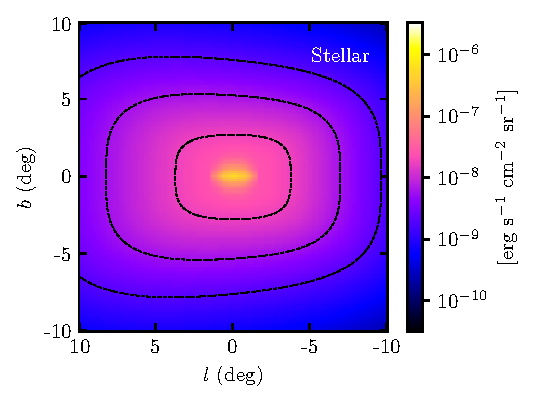
\includegraphics[width = \columnwidth]{Figures/IC_MSPs/injection_skymap_bulge.pdf}
  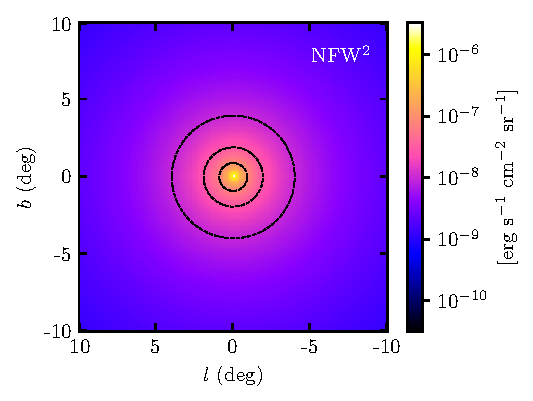
\includegraphics[width = \columnwidth]{Figures/IC_MSPs/injection_skymap_nfw.pdf}
  \caption{MSP $e^\pm$ source distributions for the stellar (top panel) and the NFW$^2$ (bottom panel) template over a $20^\circ \times 20^\circ$ region around the GC. The normalizations are determined by gamma-ray luminosities through Eq.~(\ref{eq:Le}) (see text).
The source distributions are noticeably different. While the stellar template is rectangular and asymmetric due to the tilting angle between the Galactic bar's long axis and the GC-Sun direction, the NFW$^2$ template is spherically symmetric. The very bright quasielliptical region in the central few degrees in the top panel corresponds to the NB stellar component.}
  \label{fig:injection_skymap}
\end{figure}
\begin{figure}[t!]
  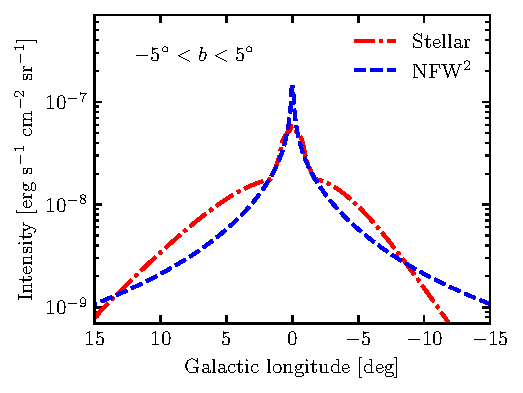
\includegraphics[width = \columnwidth]{Figures/IC_MSPs/injection_lon.pdf}
  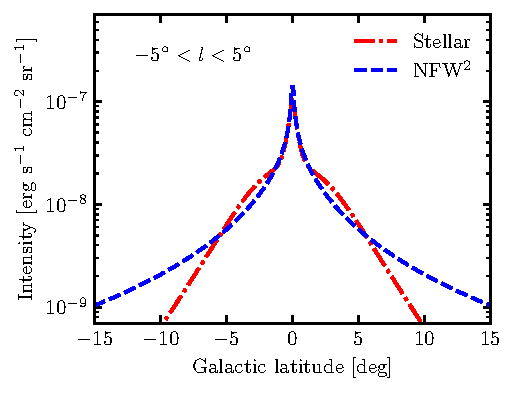
\includegraphics[width = \columnwidth]{Figures/IC_MSPs/injection_lat.pdf}
  \caption{Longitudinal (top panel) and latitudinal (bottom panel)
    profiles for the MSP $e^\pm$ source distributions considered in this work. The profiles
    are for 10$^\circ$ wide bands and show the longitude and latitude
    from $15^\circ$ to $-15^\circ$. Noticeable morphological differences are seen in both directions.}
  \label{fig:injection_profile}
\end{figure}

To show the source distribution and their relative injection intensities we produce injection intensity maps obtained by integrating along the line-of-sight direction the corresponding source density models,
\begin{equation}
  \label{eq:j_factor}
  I(l,b) \propto \int_{\text{l.o.s}} \rho(s,l,b) ds,
\end{equation}
where $l$ and $b$ are the galactic longitude and latitude and $s$ is the distance from the Sun along the line-of-sight direction.
Figure~\ref{fig:injection_skymap} (top panel) displays the injection intensities of the $\mbox{Galactic bar}+\mbox{NB}$ template in a 20$^\circ$ $\times$ 20$^\circ$ region around the GC. The resulting sky map is oblate and asymmetric. It is brighter for positive longitudes since the long axis of the bar makes a tilting angle with the GC-Sun direction. In contrast, Fig.~\ref{fig:injection_skymap} (bottom panel) shows that the NFW$^2$ source is spherically symmetric and has a strong peak in the center of the Galaxy. We also present corresponding longitudinal and latitudinal profiles for the two models in Fig.~\ref{fig:injection_profile}. The aforementioned longitudinal asymmetry in the stellar distribution can clearly be seen in the top panel. Here it is also noticeable that the NFW$^2$ intensity profile is more strongly peaked than the stellar template. The oblateness of the $\mbox{Galactic bar}+\mbox{NB}$ model is made manifest by comparing the tails of the profiles in both panels.

\subsection{Injection spectrum}\label{sec:spectrum}

The maximum energy that MSPs can accelerate $e^{\pm}$ to is estimated to be $\sim 100$ TeV. In this work we adopt a similar $e^\pm$ spectrum to that used in Ref.~\cite{Yuan:2014yda} and explore a range of parameter values. Namely, we use a power law with an exponential cutoff,
\begin{equation}
  \label{eq:msp_spectrum}
  \dfrac{dN}{dEdt} \propto E^{-\Gamma}\exp(-E/E_{\text{cut}}),
\end{equation}
where $\Gamma$ is the spectral slope and $E_{\text{cut}}$ is the energy cutoff. We vary $\Gamma$ between 1.5 and 2.5, while $E_{\text{cut}}$ is varied between 10 and 100 TeV. The combinations of spectral parameters assumed in this work are listed in Table~\ref{tab:msp_spectrum}. Note that our choice of spectral parameters represents the entire MSP population in the Galactic bulge.
\begin{table}[t!]
  \centering
  \caption{Injection spectral parameters of MSP $e^{\pm}$ adopted in this work. See Eq.~(\ref{eq:msp_spectrum}).}
    \begin{tabular}{lcc}\hline\hline
    Model Name&$\Gamma$ & $E_{\text{cut}}$\\
    & &  (TeV) \\\hline
    Baseline &2.0 & 50 \\
    Inj1&1.5 & 50 \\
    Inj2&2.5 & 50 \\
    Inj3&2.0 & 10 \\
    Inj4&2.0 & 100\\\hline\hline
    \end{tabular}
  \label{tab:msp_spectrum}
\end{table}

\subsection{Configurations}

In order to make simulations of CR propagation that are as realistic as possible, it is crucial to understand the diffusion parameters for all the CR species. Reference~\cite{Johannesson:2016rlh} performed a scan of the parameter space of the CR injection and propagation. The scan was done separately for the low-mass isotopes ($p$, $\bar{p}$ and He) and the light elements (Be, B, C, N, O). Since each set of species has a different lifetime they probe different regions of the Galaxy. They found that the best-fit parameter setup for the low mass isotopes is different from that obtained for the heavier elements. Here, we adopt the propagation parameters for the low-mass isotopes of Ref.~\cite{Johannesson:2016rlh}. We account for uncertainties in the propagation parameters by also including the 95\% credible contours provided in their 2D marginalized posterior distributions. The propagation setups used in this work are listed in Table~\ref{tab:dpara}.

We perform 3D \texttt{GALPROP} simulations using the standard ISRF data available with version 54 of the software package. The calculations are made for a Cartesian spatial grid with the Galactic plane placed in the $X$-$Y$ plane and the GC located at the origin of the coordinate system. The $X$ axis is defined by the GC-Sun direction.

In our simulations, the propagation volume extends to $\pm$20 kpc in both the $X$ and $Y$ direction. However, the CR halo height $z_h$ is set to different values depending on the model considered, as shown in Table~\ref{tab:dpara}. To trace the physics of the NB, we performed resolution tests for the spatial grid sizes. We fixed $\Delta Z$ = 0.125 kpc and found that the IC spectra and sky maps showed little difference when the resolution was $\Delta X$ = $\Delta Y$ = 0.125 or 0.25 kpc. We therefore adopted $\Delta X$ = $\Delta Y$ = $\Delta Z$ = 0.125 kpc for all our runs except for the $z_h = 19.28$ kpc run, which was performed at a lower resolution of $\Delta X$ = $\Delta Y$ = 0.25 and $\Delta Z$ = 0.125 kpc due to computing memory demands. As a result, each run takes about 80 hours to finish using a computer cluster node with 500 GB memory and running at $\sim 6 \times 10^{11}$ flop/s.

After choosing the resolution, Eq.~(\ref{eq:rhobar}) can be converted to the number of MSPs per spatial bin and normalized to reproduce the total number of MSPs that inhabit the Galactic bulge~($\sim 10^4$ \cite{Gonthier:2018ymi}). We find that every (0.125 kpc)$^3$ bin corresponds to $\sim 40$ MSPs at the GC, and $\sim 4$ MSPs at 3 kpc along the long axis of the Galactic bar. We thus approximate the MSP distribution as a smooth function in our simulations.

\begin{table}[t!]
  \centering
  \caption{\label{tab:dpara} Propagation parameter setups considered in this study. Our baseline model corresponds to the best-fit propagation parameter in the scan for low-mass isotopes in Ref.~\cite{Johannesson:2016rlh}, while the five additional models reflect the 95\% confidence contours in their propagation parameter scan \cite{Johannesson:2016rlh} (see text).}
  % \begin{ruledtabular}
    \begin{tabular}{ c c c c c }
      & $D_0$ & $z_h$ & $v_A$  &$\delta$ \\
      & (10$^{28}$ cm$^2$ s$^{-1}$) & (kpc) & (km s$^{-1}$) & \\ \hline
      Baseline & 6.330 & 9.507 & 8.922 & 0.466 \\
      Model 1 & 3.159 & 9.507 & 8.922 & 0.466 \\
      Model 2 & 7.006 & 9.507 & 8.922 & 0.573 \\
      Model 3 & 8.072 & 9.507 & 8.922 & 0.351 \\
      Model 4 & 2.748 & 3.000 & 8.922 & 0.466 \\
      Model 5 & 7.742 & 19.280 & 8.922 & 0.466 \\
    \end{tabular}
  % \end{ruledtabular}
\end{table}

We adopt the best-fit propagation of Ref.~\cite{Johannesson:2016rlh} with the default $e^\pm$ spectrum of Ref.~\cite{Yuan:2014yda} as our baseline setup. In order to evaluate the impact of different propagation and spectral assumptions, we consider different propagation model setups in Table~\ref{tab:dpara} and the different $e^{\pm}$ injection spectra listed in Table~\ref{tab:msp_spectrum}. For our baseline spectral setup we explore all variations in propagation setup. For our baseline propagation setup we explore all $e^{\pm}$ injection spectral combinations. In all our simulations the efficiency of the MSP $e^\pm$ is fixed to $f_e^\pm$ = 0.1.

\subsection{Magnetic field}\label{sec:bfield}

We adopt the default magnetic field from \texttt{GALPROP}, which is a double-exponential function,
\begin{equation}
	B(r,z) = B_0 \exp{\left(-\dfrac{r-R_\odot}{R_0}\right)}\exp{\left(-\dfrac{z}{z_0}\right)},
\end{equation}
where $B_0 = 5\ \mu$G is the local magnetic field at the Solar System radius, and the scale parameters $R_0$ = 10 kpc, and $z_0$ = 2 kpc. The magnetic field strength of this model matches the 408 MHz synchrotron data~\cite{Strong:1998fr} and is in agreement with the total Galactic magnetic field estimates in the literature~\cite{1995ASPC...80..507H,2001SSRv...99..243B}. However, the magnetic field at the center of the Galaxy remains uncertain. In particular, a multiband modeling on scales of 400 pc about the GC has produced a lower limit of 50 $\mu$G on the magnetic field strength \cite{Crocker:2010xc}, which the default \texttt{GALPROP} magnetic field does not obey (yielding, instead, a field strength of $\sim 10\ \mu$G). To this end, we test a modified magnetic field where we set $B = 50\ \mu$G within a 400 pc region around the GC, but otherwise it matches the \texttt{GALPROP} default field everywhere else. The impacts of such a magnetic field will be discussed.

\begin{figure}[t!]
  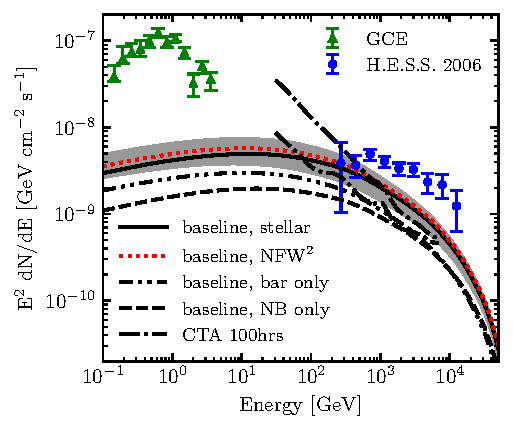
\includegraphics[width=\columnwidth]{Figures/IC_MSPs/ics_spectrum_hess_diffuse.pdf}
  \caption{IC emissions from the Galactic ridge ($6^\circ\times 2^\circ$ area around the GC). The fluxes from the baseline model for the stellar template (black solid) and NFW$^2$ template (red dotted) are shown. The shaded band represents the uncertainties due to the propagation parameters for the stellar template. The NB (dashed) and the Galactic bar (dot-dot-dashed) are shown separately for the baseline stellar model. Green triangles show the GCE data~\cite{Macias:2016nev} and blue circles show the H.E.S.S. residuals~\cite{Aharonian:2006au} in the Galactic ridge region. The upper dot-dashed (lower dot-dashed) line shows the CTA sensitivity for 100 hours from an ON-OFF analysis using the ring method toward the GC with (without) systematic uncertainty considerations~\cite{Silverwood:2014yza}. A dedicated morphological analysis could improve the shown sensitivities by up to a factor of $\sim 10$ \cite{Silverwood:2014yza}.}
  \label{fig:spectrum_diffuse}
\end{figure}

\section{\label{sec:results} Results}

Figure~\ref{fig:spectrum_diffuse} shows the predicted IC emissions from the Galactic ridge region (defined as the $6^\circ\times 2^\circ$ area around the GC) for our stellar template (Galactic bar + NB). The solid black line is the expected flux from the baseline model. The shaded band represents the uncertainties resulting from changing the propagation setups as listed in Table~\ref{tab:dpara}. In the same plot we also show the expected flux from the NFW$^2$ template (red dotted), which is indistinguishable from that from the stellar template given the uncertainties from the propagation parameters. This conclusion also holds for larger regions of the bulge of interest ($20^\circ\times 20^\circ$ around the GC). For the stellar template, we also show the IC emissions from the NB and the Galactic bar separately. For the Galactic ridge, the NB contributes $\sim 1/3$ of the total IC emission in the GeV energy range, and $\sim 1/2$ in the TeV range.

\begin{figure}[t!]
  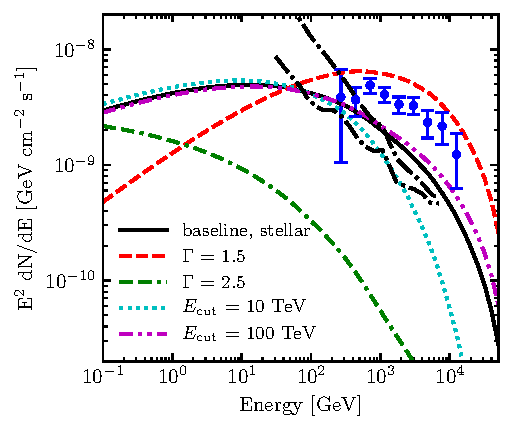
\includegraphics[width=\columnwidth]{Figures/IC_MSPs/ics_spectrum_hess_spectral.pdf}
  \caption{IC emissions for different $e^\pm$ spectra as listed in Table~\ref{tab:msp_spectrum}. H.E.S.S.~data and CTA sensitivities are shown in the same way as in Fig.~\ref{fig:spectrum_diffuse}, but note the different $y$ axis range.  Most spectra are below the H.E.S.S. measurements except for the hardest spectrum $\Gamma$ = 1.5 with $E_{\text{cut}}$ = 50 TeV which could be alleviated by a lower fraction of spin-down energy into relativistic $e^\pm$. For the soft spectrum $\Gamma$ = 2.5, the fluxes are below the CTA sensitivities by more than an order of magnitude.}
  \label{fig:spectrum_spectral}
\end{figure}

The GCE data~\cite{Macias:2014sta} at GeV energies, scaled to the Galactic ridge region, are shown by green triangles. The IC emission from MSPs is predicted to contribute less than $\sim 10$ \% of the GCE. This is consistent with previous works that have not found evidence for secondary emission at the $\sim 1$ GeV energy range~\cite{Lacroix:2015wfx}. The IC fluxes extend to the TeV energy range before decreasing steeply at $\sim 10$ TeV. Meanwhile the predicted fluxes are below or within the range of H.E.S.S.~observations (blue circles)~\cite{Aharonian:2006au}. Our resolution does not probe the smaller-scales of $0.2^\circ$--$0.5^\circ$ investigated in Ref.~\cite{Hooper:2018fih}. Also shown in the same figure are the differential sensitivities for 100 hours of CTA diffuse GC observations~\cite{Silverwood:2014yza} (dot-dashed black lines). We note that our predicted IC fluxes could be detected by forthcoming CTA observations. Reference~\cite{Silverwood:2014yza} computed the CTA sensitivities to a DM annihilation signal in the GC. Although the spatial morphology considered in their work is different than ours, we use it as a representative of the CTA sensitivities to a large diffuse signal in this sky region. That work also showed that by performing dedicated morphological analyses, the sensitivity of CTA can be improved by up to an order of magnitude for DM annihilation signals. We expect that similar improvements could be obtained by performing such morphological analyses with the models considered in our current study.

\begin{figure*}[t!]
	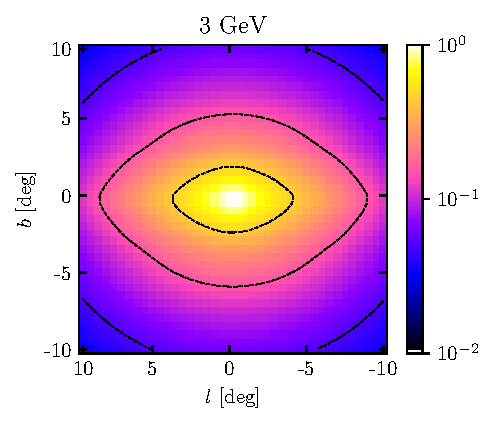
\includegraphics[width=0.68\columnwidth]{Figures/IC_MSPs/skymap_bulge_3gev.pdf}
    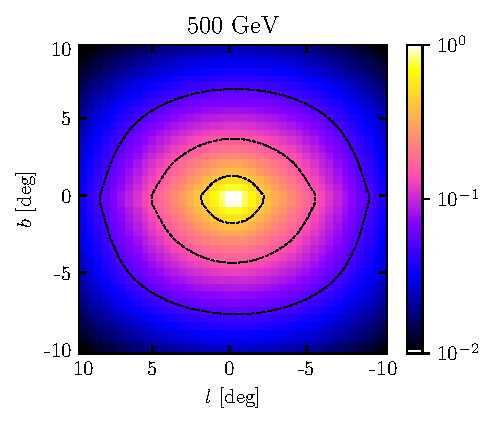
\includegraphics[width=0.68\columnwidth]{Figures/IC_MSPs/skymap_bulge_500gev.pdf}
     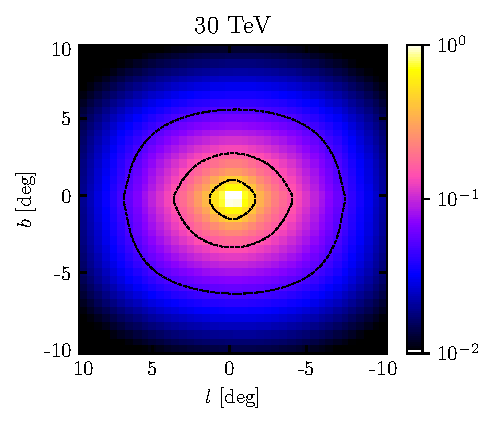
\includegraphics[width=0.68\columnwidth]{Figures/IC_MSPs/skymap_bulge_30tev.pdf}
    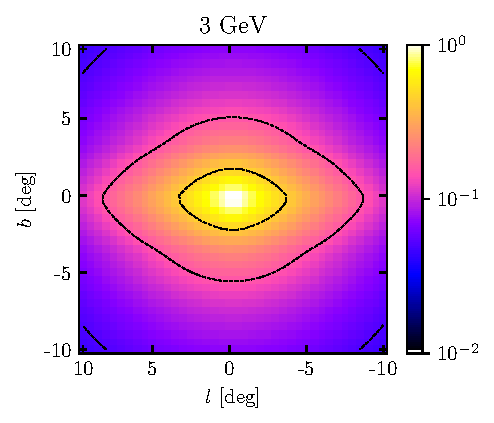
\includegraphics[width=0.68\columnwidth]{Figures/IC_MSPs/skymap_nfw_3gev.pdf}
    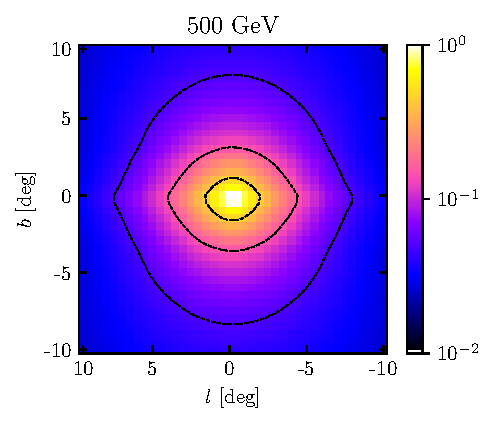
\includegraphics[width=0.68\columnwidth]{Figures/IC_MSPs/skymap_nfw_500gev.pdf}
    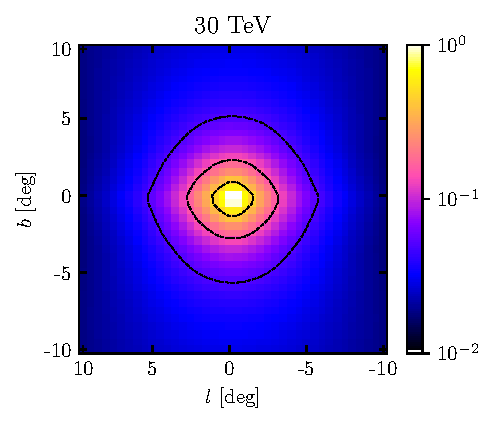
\includegraphics[width=0.68\columnwidth]{Figures/IC_MSPs/skymap_nfw_30tev.pdf}
  \caption{IC sky maps from the baseline model for the stellar template (top row) and the NFW$^2$ template (bottom row) over a $20^\circ\times 20^\circ$ region around the GC. Three energy windows are shown: 3 GeV (left column), 500 GeV (center column), and 30 TeV (right column). The injected $e^\pm$ are normalized by gamma-ray luminosities. The 5\%, 15\%, and 45\% flux levels with respect to the GC are shown by dotted contours. The morphological differences between the stellar template and the NFW$^2$ template appear more prominently at high energies.}
  \label{fig:skymap_bulge_vs_nfw}
	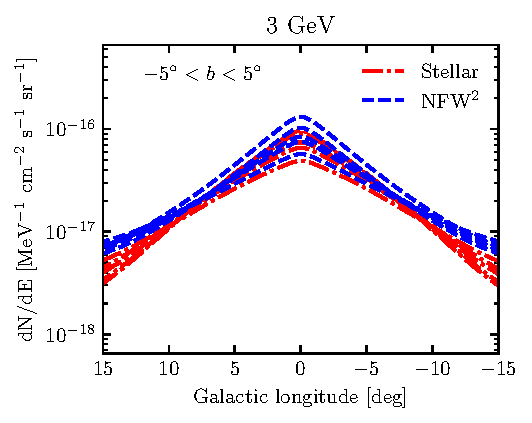
\includegraphics[width=0.68\columnwidth]{Figures/IC_MSPs/lon_3gev.pdf}
    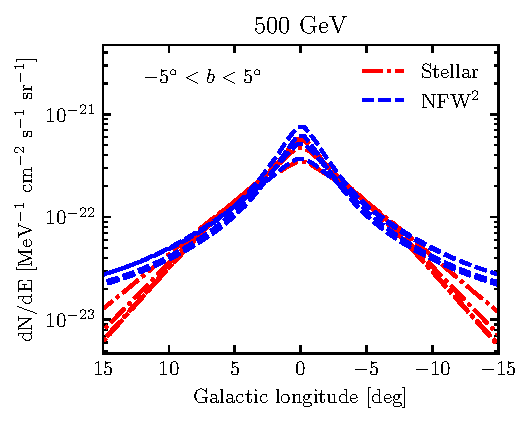
\includegraphics[width=0.68\columnwidth]{Figures/IC_MSPs/lon_500gev.pdf}
	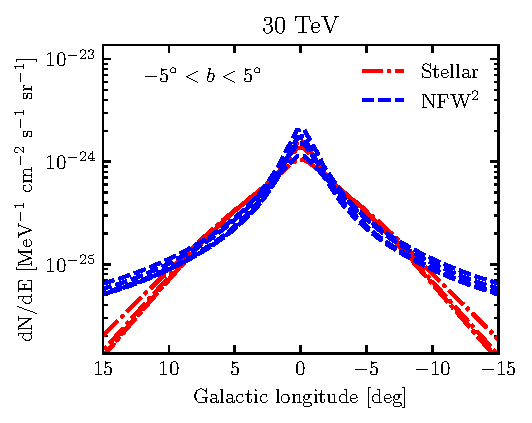
\includegraphics[width=0.68\columnwidth]{Figures/IC_MSPs/lon_30tev.pdf}
	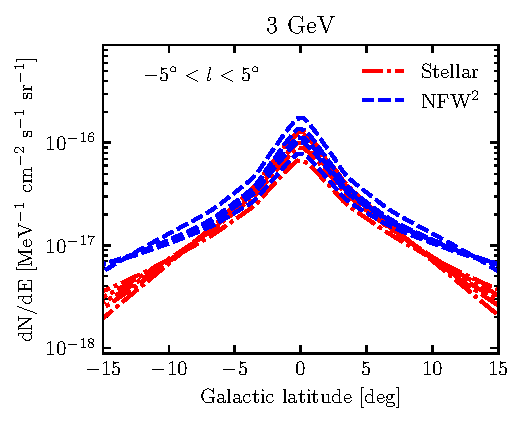
\includegraphics[width=0.68\columnwidth]{Figures/IC_MSPs/lat_3gev.pdf}
	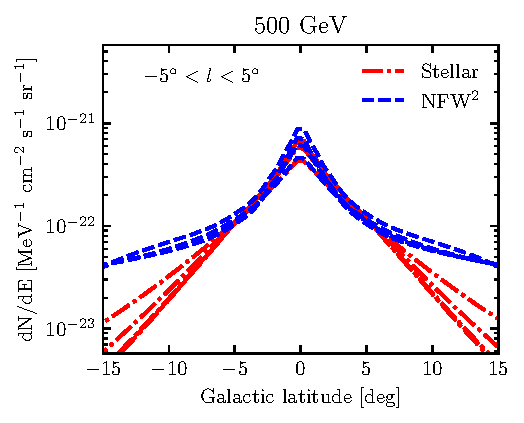
\includegraphics[width=0.68\columnwidth]{Figures/IC_MSPs/lat_500gev.pdf}
	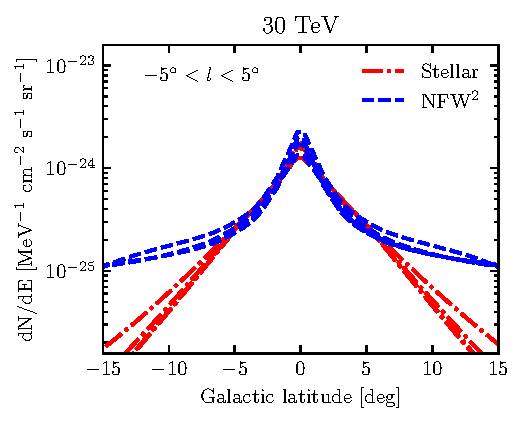
\includegraphics[width=0.68\columnwidth]{Figures/IC_MSPs/lat_30tev.pdf}
  \caption{IC longitudinal (top row) and latitudinal (bottom row) profiles for the stellar template (red dot-dashed) and NFW$^2$ template (blue dashed), showing predictions from different propagation models as listed in Table~\ref{tab:dpara}.  The profiles are obtained by summing over 10$^\circ$ wide bands in the latitude and longitude directions, respectively. The columns are for the same energy windows as in Fig.~\ref{fig:skymap_bulge_vs_nfw}. The profiles show consistent changes in energy as seen in the corresponding sky map, and that the differences between the stellar and NFW$^2$ templates are greater than the differences caused by our selection of propagation setup.}
  \label{fig:profile_bulge_vs_nfw}
\end{figure*}

The IC spectra from the Galactic ridge region for different MSP injection spectra (Inj1, Inj2, ..., Inj4) are shown in Fig.~\ref{fig:spectrum_spectral}. We find that most of our predictions are at or below the corresponding H.E.S.S.~data points (assuming $f_{e^\pm} = 10\%$). However, for the hard injection spectrum model Inj1 ($\Gamma = 1.5$ and $E_{\text{cut}}=50$ TeV), the IC spectra overshoots the H.E.S.S.~observations. This means that either the Inj1 model is disfavored, or that $f_{e^\pm}$ is lower than $\sim 6\%$ in the Galactic ridge region. Contributing to this overshooting could be that the $e^\pm$ injection in the NB is overestimated. This is due to the fact that we normalize the $e^\pm$ luminosity by their gamma-ray luminosities. The best-fit NB gamma-ray luminosity obtained by Ref.~\cite{Macias:2016nev} may be somewhat overestimated, because the NB spatial morphology is similar to that of the CMZ structure which could cause spatial degeneracies in the fits. In this sense, a fraction of the gamma-ray photons that are of hadronic origin (emitted by the CMZ) could have been absorbed by the NB stellar template. Also, we note that at around 100 TeV, pair production will attenuate the predicted flux by $\sim 3/4$.

\begin{figure}[t!]
  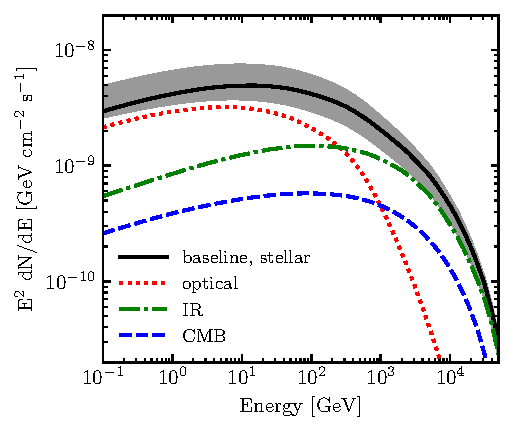
\includegraphics[width=\columnwidth]{Figures/IC_MSPs/ics_spectrum_components.pdf}
  \caption{Components of the IC emission for the baseline stellar model from the Galactic ridge, arising from different up-scattered photon fields: optical (red dotted), IR (green dot-dashed), CMB (blue dashed), and the total (black solid). The optical component dominates the GeV energy range, but decreases above 100 GeV, eventually being overtaken by up-scattered IR and CMB photons.}
  \label{fig:spectrum_comp}
\end{figure}

Figure \ref{fig:skymap_bulge_vs_nfw} shows the morphologies of the IC emission for our baseline models in different energy windows: 3 GeV (left), 500 GeV (center), and 30 TeV (right). The top (bottom) row shows the sky maps for the stellar (NFW$^2$) template. The sky maps are normalized by their fluxes at the GC. We find that there are energy-dependent morphological differences between the two IC predictions. These reflect the different $e^\pm$ source distribution models considered. In the GCE energy range ($\sim 3$ GeV, left panels), the IC sky maps are similarly elliptical for both the stellar and NFW$^2$ templates. However, the sky maps become less elliptical at 500 GeV and above. At around $\sim 30$ TeV, the morphologies of the IC component start to show the source distributions displayed in Fig.~\ref{fig:injection_skymap}. As it can be seen, in the highest energy window the sky maps for the stellar template (top-right panel) are boxy while that for the NFW$^2$ template (bottom-right panel) is close to spherical. However, the left-right asymmetry due to the tilt of the bar is not seen in the IC emissions.

These features can be seen more clearly in the corresponding latitudinal and longitudinal profiles presented in Fig.~\ref{fig:profile_bulge_vs_nfw}. Here, we also show the variations in predicted IC morphologies when the propagation setups are varied, as in Table~\ref{tab:dpara}. We note that the morphological differences between the stellar and NFW$^2$ templates are robust to changes in the propagation parameters. It is clear that at tens of TeV, the IC sky maps are sensitive to the source injection distributions.

\begin{figure}[t!]
  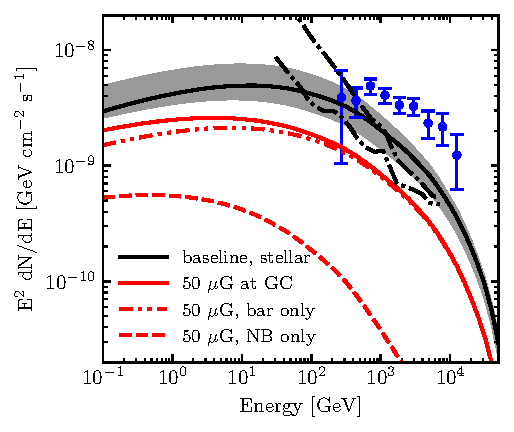
\includegraphics[width=\columnwidth]{Figures/IC_MSPs/ics_spectrum_bfields.pdf}
  \caption{IC emissions from different magnetic field models. The baseline (black solid curve) adopts the original \texttt{GALPROP} magnetic field. The red solid curve introduces a 50 $\mu$G lower limit for the inner 400 pc region around the GC. With the presence of such a lower limit, the IC emission from the Galactic ridge is reduced by $\sim 1/2$. Due to the higher overlap with the modified magnetic field, the IC emission from the NB (red dashed curve) is suppressed more strongly by synchrotron loss compared to the Galactic bar (red dot-dot-dashed curve).}
  \label{fig:spectrum_bfields}
\end{figure}

At IC photon energies of $\sim 1$ GeV, the IC emission is in the nonrelativistic (Thomson) regime and the IC flux is dominated by up-scattered optical photons (Fig.~\ref{fig:spectrum_comp}). The optical photons are mainly emitted by stars whose density peaks along the Galactic plane. As a result, in this energy range the IC emissions are elongated along the Galactic plane and have marked elliptical appearances. This is almost invariant of the spatial morphology of the MSP distributions assumed, explaining the similarity between the left panels of Fig.~\ref{fig:skymap_bulge_vs_nfw}. However, at higher energies, the IC emission starts to enter the relativistic scattering (Klein-Nishina) regime and becomes suppressed, causing the decline of the up-scattered optical photon signal from around 100 GeV (red dotted curve in Fig.~\ref{fig:spectrum_comp}). Since the Klein-Nishina regime is reached at higher energies for lower-energy target photons~\cite{Fermi-LAT:2014sfa}, the IR and CMB photons continue, overtaking the optical photons. Furthermore, as the IR is less concentrated along the Galactic plane than the optical photons (and the CMB is isotropic), the IC emission retains more morphological information of the injected $e^\pm$.

A larger magnetic field means greater energy loss due to synchrotron radiation of the injected $e^\pm$ and a corresponding reduction in the IC emission. We tested a constant magnetic field $B = 50\ \mu$G in the GC region on scales of 400 pc (see Sec.~\ref{sec:bfield}) to explore its impact on our model predictions. Figure~\ref{fig:spectrum_bfields} shows the predicted IC spectrum for the baseline model assuming the default magnetic field (black solid curve with gray shaded band) and the corresponding IC spectrum for the same model but assuming the modified magnetic field (red solid curve). As can be seen, the IC spectrum normalization for the enhanced magnetic field setup is $\sim 1/2$ of the default one. This represents a change in normalization that is larger than our estimated modeling uncertainties from different propagation models (gray shaded). This reduction is mainly due to synchrotron energy loss of $e^\pm$ in the NB. Figure~\ref{fig:spectrum_bfields}  displays the predicted IC spectrum for the NB component (red dashed curve) and Galactic bar (red dot-dot-dashed curve) separately in the enhanced magnetic field case. We observe that for this case the Galactic bar emission dominates. This is different to our predictions obtained using the default magnetic field setup, where the NB and bar  contributions were comparable (see Fig.~\ref{fig:spectrum_diffuse}). This can be understood by noticing that the NB resides in the region where the modified magnetic field underwent the normalization increase. Consequently, much of the $e^\pm$ emitted from this region endure maximum energy loss via synchrotron radiation.

\section{\label{sec:conclu}Discussion and Conclusion}

Recent analyses of the GCE~\cite{Macias:2016nev,Bartels:2017vsx,Macias:2019omb} have revealed its nonspherical nature and have provided further support for an MSP origin. We have revisited the computation of secondary IC emission from the $e^\pm$ injected by such MSPs. Compared to previous studies that assumed a spherically symmetric spatial distribution of MSPs, we adopted 3D models of the stellar distributions in the GC and numerically calculated the IC emissions using the {\tt GALPROP} code. Furthermore, we systematically explored the impact of diffusion parameter uncertainties with additional {\tt GALPROP} runs. We found that the predicted IC fluxes beyond 100 GeV are within the forecasted sensitivity limits of future gamma-ray telescopes for our baseline parameters (Fig.~\ref{fig:spectrum_diffuse}). The very high-energy IC emission from MSPs is nondegenerate with that caused by DM annihilation, from which the $e^\pm$ can only reach a few tens of GeV if DM is responsible for the GCE.

Although the IC spectra from the GC provide insufficient information for identifying the spatial model of the source, we found that the spatial morphology of the IC could serve as a discriminant between the spherically symmetric and 3D stellar distribution injection models (Fig.~\ref{fig:skymap_bulge_vs_nfw}). In the GeV energy range, the IC morphologies are equally elliptical for both the stellar and NFW$^2$ models. However, above $\sim$ TeV energies, they reveal morphological differences that trace the injection distributions. They can therefore be used to discriminate the spherically symmetric and 3D stellar injection models.

Our predicted IC fluxes contribute $\lesssim 10 \%$ of the GCE emission and are at or below than the H.E.S.S.~observations of the Galactic ridge at around a  few TeV. These are consistent with the null detection of secondary emissions in the GeV range \cite{Lacroix:2015wfx} and the dominantly hadronic origins of the H.E.S.S.~measurements ~\cite{Gaggero:2017jts,Abramowski:2016mir}. Thus they constitute important consistency checks of the MSP scenario for the GCE. We compared the IC fluxes with the CTA sensitivity from Ref.~\cite{Silverwood:2014yza} and found that the IC emission could be detected and potentially reveal a signature of GC MSPs with a specialized spectral and morphological search. The HAWC telescope~\cite{DeYoung:2012mj,Abeysekara:2013tka} operates in similar energy bands, and while not having a full view of the Galactic bulge region may have sensitivity to hard $e^\pm$ injection models. To this end, a wide field-of-view TeV gamma-ray observatory in the southern hemisphere is warranted \cite{Mostafa:2017fza}.

The detectability of the IC emission depends on the setup, including MSP $e^\pm$ spectrum and propagation parameters. We adopted a canonical $e^\pm$ power-law slope of 2.0, but softer spectra would make it a challenge to detect the IC component at TeV energies (Fig.~\ref{fig:spectrum_spectral}). Furthermore, an increased magnetic field at the GC would reduce the IC emission via enhanced synchrotron energy losses. In particular, assuming a constant magnetic field of magnitude 50 $\mu$G in the inner 400 pc of the GC, we found a reduction of $\sim 1/2$ of the IC emission obtained with the default magnetic field setup. On the other hand, our model predictions were not very sensitive to changes in the propagation parameters within the 95\% credible contours provided in the 2D marginalized posterior distributions of Ref.~\cite{Johannesson:2016rlh}.

There are various assumptions in our calculations that warrant future detailed studies. For example, we used the default ISRF from the {\tt GALPROP} version 54, which is 2D after averaging the angular dependence. This has recently been updated in Refs.~\cite{Porter:2017vaa,Johannesson:2018bit}, where a 3D ISRF was adopted in the context of CR propagation and high-energy gamma-ray emissions in the Galaxy. Their results show nontrivial impacts from employing the 3D ISRF on the propagation parameters of CRs and the gamma-ray intensity maps. Our results may be affected in many ways, including the fluxes and sky maps. Studies with the {\tt PICARD} code show that new ISRFs increase gamma-ray intensities from the Galactic center, in particular at energies of $\sim 200 $ GeV \cite{Niederwanger:2018zsv}. Note however that our Galactic bar parametrization remains consistent with the ISRF of {\tt GALPROP}. Even though more recent analyses suggest a larger tilt angle, we found that the left-right bulge asymmetry caused by the tilt is washed out in the IC sky maps, and is certainly smaller than the uncertainty caused by propagation parameters.

For the propagation part, we have adopted the results of a wide scan of propagation parameters \cite{Johannesson:2016rlh}. However, caution must be exercised since the propagation properties around the Galactic center may be unique. We also have not covered all possibilities, e.g., we did not consider the possibility of cosmic rays advected out of the region by large-scale outflows. Such outflows may be related to the Fermi bubbles \cite{Crocker:2014fla} and depending on the velocity would affect the secondary IC morphology. We have also neglected MSPs in the Galactic disk, which would provide additional $e^\pm$ injection and IC emission. However, population syntheses show that the MSP contribution to the Galactic diffuse gamma-ray emission is at the few-percent level or less \cite{Gonthier:2018ymi} and we do not expect this to substantially affect our results.

We have modeled the MSP population in the Galactic bulge. However, the presence of younger pulsars and the evolution of the pulsar population were not considered. It has been shown that TeV halos from younger pulsars can contribute to TeV emissions~\cite{Hooper:2017rzt}. This may potentially change the spectral property of IC emissions from the NB where active star formation is ongoing.

The magnetic field at the GC is a crucial parameter affecting the IC emission from a putative MSP population in the nuclear bulge. We have shown that an enhanced magnetic field in this region in turn augments the synchrotron energy losses of the MSP $e^\pm$, thus decreasing the IC yields. The estimated magnetic fields at $\sim$ 100 pc around the GC has large uncertainties and vary from 10 $\mu$G~\cite{LaRosa:2005ai} to 1000 $\mu$G~\cite{Morris1989fd}. Here we only tested the original \texttt{GALPROP} model ($\sim 10\ \mu$G at the GC) and a 50 $\mu$G lower limit obtained in Ref.~\cite{Crocker:2010xc}. An even larger magnetic field at the GC means that the synchrotron radiation would be dominant, especially for the NB component that resides within the 230 pc region around the GC. The spectrum and morphology of the IC emission from the Galactic ridge would potentially be changed by a strong magnetic field in this region. However, the effects on the larger-scale bar/bulge component are expected to be minor. On the other hand, we have only considered the 2D random magnetic field component. A recent study~\cite{Orlando:2019vmq} showed that the IC spatial maps can be significantly affected when more realistic 3D magnetic fields with both random and ordered components are included. This will apply also in the context of MSP secondary emission but its investigation is beyond the scope of the current study.

The Galactic center of the Milky Way offers a unique window to study novel astrophysical and dark matter signals. We have shown that the TeV energy range offers a new handle on the morphology of putative MSPs in the Galactic bulge responsible for the GeV excess. Telescopes such as CTA and HAWC South can be helpful for detecting these IC emissions and for constraining the origin of the GCE in the future.

\chapter{Gamma rays from globular clusters} \label{ch:globular_cluster}

\section{Introduction}\label{sec:intro}

Over two dozen globular clusters (GCs) have been detected in $\gamma$ rays in {\it Fermi} Large Area Telescope (LAT) data~\citep{2009Sci...325..845A,2010A&A...524A..75A,2010ApJ...712L..36K,2011ApJ...729...90T,2015MNRAS.448.3215Z,2016MNRAS.459...99Z}. The millisecond pulsar (MSP) populations of those GCs are believed to be the main source of this $\gamma$-ray emission. In particular, MSPs have been firmly established as $\gamma$-ray sources~\citep{1996A&A...311L...9V,2009ApJ...699.1171A,2013MNRAS.430..571E,2013ApJS..208...17A} and a large fraction of them have been discovered in GCs~\citep{2005ASPC..328..147C}. Recently, \textit{Fermi}-LAT detected $\gamma$-ray pulsations in two GCs~\citep{2011Sci...334.1107F,2013ApJ...778..106J}, providing further support for this scenario.

The high-energy emission from MSPs emerges from the primary electrons accelerated by them and  subsequent radiation by secondary, relativistic electrons and positrons ($e^\pm$) pair created in their magnetospheres. In particular, \citet{2005ApJ...622..531H} studied the curvature radiation (CR) of primary electrons within MSP magnetospheres with a focus on GeV-scale emission. \citet{2007MNRAS.377..920B} then considered a scenario in which $e^\pm$, injected by MSPs, gradually diffuse through a GC, up-scattering ambient photons, and thus producing inverse Compton (IC) $\gamma$-ray emission in the GeV$-$TeV energy range.~\citet{2009ApJ...696L..52V} calculated the CR and IC spectra for an ensemble of MSPs in the GCs 47 Tucanae and Terzan 5. \citet{2010ApJ...723.1219C} found that the spectra of 47 Tucanae and seven other GCs can be explained by IC alone, invoking background photons from the cosmic microwave background (CMB) or Galactic infrared/stellar radiation. {For a review of the observations and models about the $\gamma$-ray emission from globular clusters, see \citet{2016JASS...33....1T}.} In general, the GeV emission mechanism of MSPs remains in contention with CR, IC, and synchrotron radiation all  proposed~\citep{2021arXiv210105751H}.

Here, motivated by the increasing number of GCs detected in $\gamma$ rays, we perform a collective statistical study of their properties in order to gain insight into the nature of their high-energy emission. Our particular aim is to investigate the importance of the contribution of IC emission to the overall $\gamma$-ray emission of GCs.

Relations between the detected GC gamma-ray luminosities and properties of GC can be used to probe the origins of $\gamma$-ray emission and their underlying sources. For example, correlations with the photon field energy density of GCs could unveil the potential contribution from IC, and correlations with the stellar encounter rate and metallicity could provide insight into the dynamical formation of MPSs in GCs. Previous work here includes a study by \citet{2010A&A...524A..75A} that reported a correlation between the $\gamma$-ray luminosity $L_\gamma$ and the stellar encounter rate of eight GCs. \citet{2011ApJ...726..100H} studied a group of 15 $\gamma$-ray emitting GCs with 2 years of Fermi data and found a positive correlation between $L_\gamma$ and, respectively, encounter rate, metallicity, and Galactic photon energy density. \citet{2016JCAP...08..018H} studied 25 GCs using 85 months of Fermi data, and found that the $\gamma$-ray luminosity function of MSPs in GCs is consistent with that applying to MSPs detected in the field. \citet{2018MNRAS.480.4782L} studied $\gamma$-ray emission from high-latitude GCs and its connection to their X-ray emission. \citet{2019MNRAS.486..851D} reanalysed 9 years of Fermi data and found 23 $\gamma$-ray emitting GCs; they found that the metallicity only mildly contributes to $L_\gamma$ while a very high encounter rate seemed to {\it reduce} the $L_\gamma$ from GCs.

In parallel, modeling of GCs' observed broadband spectral energy distributions provides a handle on their CR and IC emissions. Recently,~\citet{2013ApJ...779..126K} and~\citet{2019ApJ...880...53N} modelled the multiwavelength emission from MSPs considering a potential CR origin for GeV and IC emissions for TeV $\gamma$ rays, as well as synchrotron radiation for the radio and X-ray wavebands. These models are successful in explaining the multiwavelength spectra of Terzan 5. However, Terzan 5 is the only GC (perhaps) detected above TeV energies~\citep{2011A&A...531L..18H}. Detailed spectral modelling similar to that presented by~\citet{2013ApJ...779..126K} and~\citet{2019ApJ...880...53N} is difficult for other GCs at present due to a lack of TeV $\gamma$-ray data. Although \textit{Fermi}-LAT is sensitive to $\gamma$-rays of up to $\approx 1$ TeV, the photon count statistics at the highest energies are very low.

In the recently published \textit{Fermi}-LAT fourth source catalog~\citep{2020ApJS..247...33A} (4FGL)\footnote{The Fermi collaboration has recently released an incremental update of the fourth source catalog~\citep{2020arXiv200511208B} (4FGL-DR2, for Data Release 2). The new catalog uses 10 years of data, a 25\% increase with respect to the 4FGL. However, only 1 new GC (NGC 362) has been detected. Given this marginal change, we retain use of the 4FGL catalog constructed with the 8-year data set.}, 30 GCs have been detected in GeV $\gamma$ rays. With such a number, we can begin to carefully study the nature of the $\gamma$-ray emission from GCs through a population study. In this paper, we repeat the bin-by-bin analysis of the 4FGL data for the 157 known Milky Way GCs in the \citet{1996AJ....112.1487H} catalog\footnote{2010  edition: \url{https://www.physics.mcmaster.ca/~harris/mwgc.dat}}. We search for correlations between the $\gamma$-ray luminosity of the GCs and other parameters of the GCs to probe which are good proxies for the $\gamma$-ray luminosity and study potential IC contributions; to this end, we consider the photon field energy densities, the stellar encounter rate, and the metallicity of the GCs. Unlike previous studies of correlations of the GC $\gamma$-ray emissions, we consider also the upper limits placed by null detections, which we implement via a Kendall $\tau$ coefficient test statistic. Furthermore, we also look for evidence of IC from the spectra of GCs. For the first time, we implement a universal two-component model to study the spectra of $\gamma$-ray-detected GCs. The two-component model comprises a CR component, which is spectrally curved, plus an IC component modeled as a power law in the energy range of interest.

The remainder of the paper is as follows: In Section~\ref{sec:gamma_GCs} we discuss the choice of GC samples and the data analysis procedure. Section~\ref{sec:correlation} presents the methodology and results of our correlation analysis. Section~\ref{sec:spectra} describes the spectral analysis method and reports the $e^\pm$ injection efficiency in the GCs. We discuss the implications of our results in Section~\ref{sec:discussion} and conclude in Section~\ref{sec:conclusion}.

\section{$\gamma$-ray emission from globular clusters}\label{sec:gamma_GCs}

In this section, we describe our choice of GC sample and the GCs' $\gamma$-ray-related parameters. The Fermi data analysis process is reported as well. For GCs with a $\gamma$-ray counterpart in the 4FGL, we update their spectral parameters through a maximum likelihood procedure. For those not detected in the 4FGL, we estimate their 95\% C.L. $\gamma$-ray upper limits.

\subsection{Globular cluster sample}\label{sec:samples}

We consider the \citet{1996AJ....112.1487H} catalog (2010 edition), which contains identifications and basic parameters for 157 GCs in the Milky Way. Here, we reanalyse publicly available {\it Fermi}-LAT data from the direction of all GCs in the \citet{1996AJ....112.1487H} catalog. Figure~\ref{fig:all_sky_distribution} shows the spatial distribution of the GCs. The top panel shows the projected direction of the GCs on the celestial plane while the bottom two panels display their 3D coordinates. The GCs which are detected in the 4FGL are marked by red stars while null detections are indicated by green circles. Most $\gamma$-ray GCs are near the Sun (yellow circle) or located in the Galactic bulge (assumed to be sphere of 3 kpc radius, grey circular area).

\begin{figure}
    \centering
    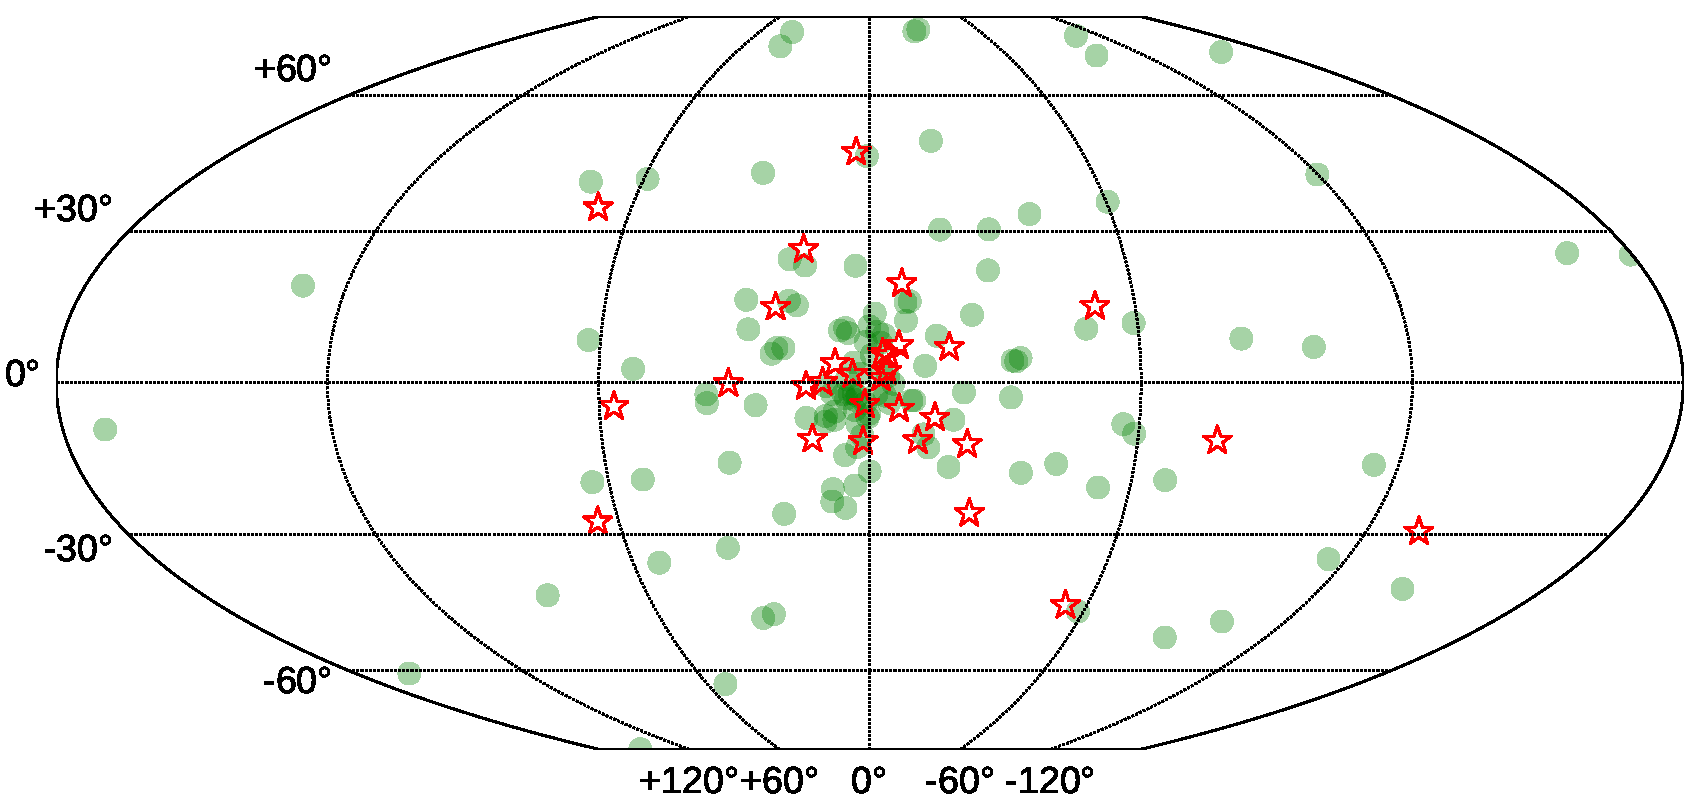
\includegraphics[width=\columnwidth]{Figures/Globular/AllSky_map.pdf} \\
    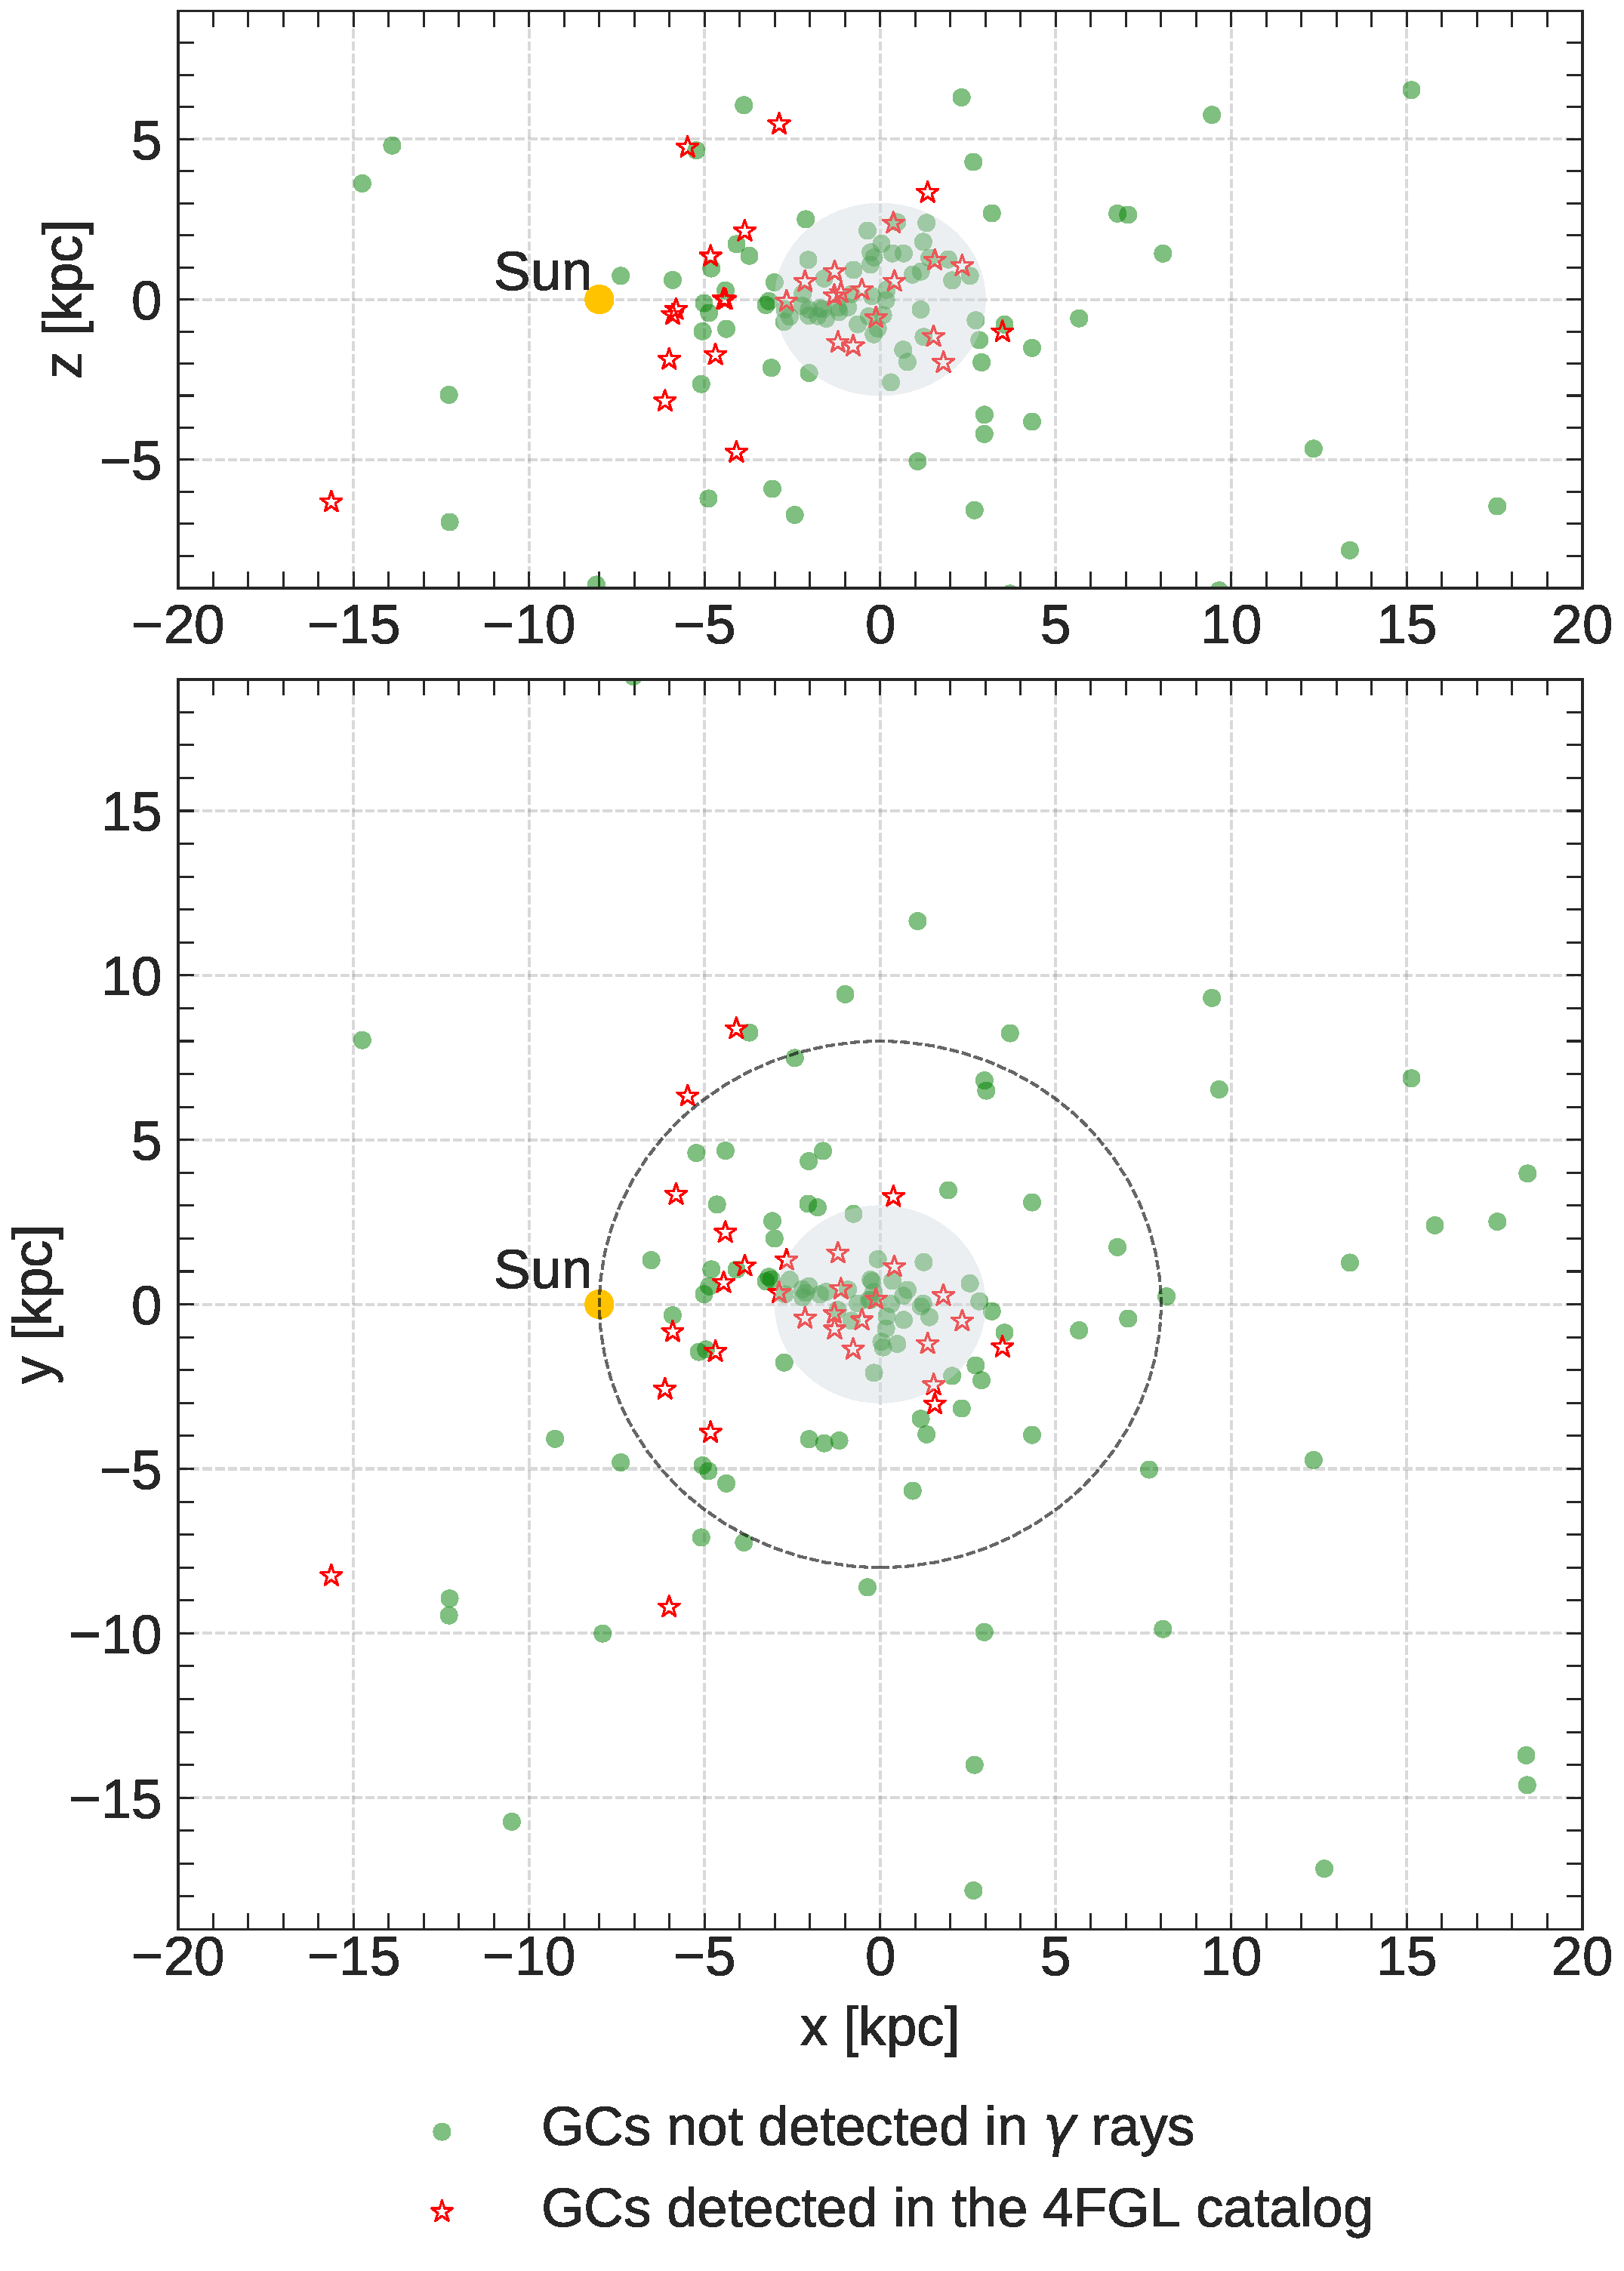
\includegraphics[width=\columnwidth]{Figures/Globular/distance_map.pdf}
    \caption{Spatial distribution of the 157 Milky Way GCs in the \citet{1996AJ....112.1487H} catalog. The top panel shows  the all sky spatial distribution in Galactic coordinate. The middle and bottom panel display the three-dimensional (3D) Cartesian %are in the 3D 
    coordinates of the GCs, in which %where 
    the Sun (yellow circle) is located in the negative x-axis. The $\gamma$-ray-detected GCs in the 4FGL catalog are shown as red stars, %and those
    and the GCs not detected in $\gamma$ rays are shown as green circles. Most $\gamma$-ray-detected GCs are located near the Sun or in the Galactic bulge (grey shaded area in the middle and bottom panel).}
    \label{fig:all_sky_distribution}
\end{figure}

The origin of the $\gamma$-ray emission from GCs can be studied by comparing its dependency on GC properties. IC emission is sensitive to the ambient photon field on which the $e^\pm$ scatter. \citet{2011ApJ...726..100H} reported a positive correlation between the $\gamma$-ray luminosity $L_\gamma$ and the photon field energy density at the cluster location, indicating an IC contribution. In the present work, we improve upon the Galactic radiation field model used by \citet{2011ApJ...726..100H} by extracting the energy density of the interstellar radiation at the locations of the GCs from the three-dimensional interstellar radiation model in \texttt{GALPROP v56}\footnote{\url{http://galprop.stanford.edu/}}~\citep{2017ApJ...846...67P,2018ApJ...856...45J}. This is a fully 3D model that combines the CMB, infrared, and optical photons of the Milky Way, denoted as $u_\text{MW}$. In addition, photons from stars in the GCs are expected to make a dominant contribution to the total, ambient radiation field. We estimate this component by
\begin{equation}
    u_{\text{GC}} = \dfrac{L_*}{4\pi c r_h^2},
    \label{eq:GCRF}
\end{equation}
where $L_*$ and $r_h$ are the stellar luminosity and the half-light radius of the GC. The total photon field energy density is $u_\text{Total} = u_\text{MW} + u_\text{GC}$.

A potential correlation between the $\gamma$-ray luminosity $L_\gamma$ and the stellar encounter rate has been studied as a way to probe the dynamic formation of MSPs in GCs~\citep{2010A&A...524A..75A,2011ApJ...726..100H,2019MNRAS.486..851D}. In the present work, we adopt the stellar encounter rate estimated by \citet{2013ApJ...766..136B}, which is defined as
\begin{equation}
    \Gamma_c = \frac{4\pi}{\sigma_c}\int\rho(r)^2 r^2dr,
	\label{eq:encounter}
\end{equation}
where $\sigma_c$ is the velocity dispersion at the core radius, $\rho(r)$ is the stellar density profile of the cluster, and the line-of-sight integration is performed along the half-light radius. 

Additionally, it has been argued~\citep{2011ApJ...726..100H,2019MNRAS.486..851D} that high metallicity [Fe/H] in the GCs could enhance the dynamical formation of MSP. The outer convective zone of metal-rich stars enables magnetic braking, which assists orbital shrinking during binary formation. In this analysis, we use the GCs metallicities  reported in the~\citet{1996AJ....112.1487H} catalog, which summarizes  spectroscopic or photometric estimates in the literature.

In summary, we consider the empirical dependence of the inferred $\gamma$-ray luminosity of GCs on four parameters, namely, $u_\text{MW}$, $u_\text{Total}$, $\Gamma_c$, and [Fe/H]. We summarize the values of these parameters for the 30 $\gamma$-ray-detected GCs in Table~\ref{tab:pars}. Also included are the stellar masses M$_*$ of the GCs adopted from~\citet{2017MNRAS.464.2174B},~\cite{2017MNRAS.471.3668S}, and~\citet{2018MNRAS.478.1520B}. They are estimated from N-body modelling of the velocity dispersion and surface density profiles. In Section~\ref{sec:correlation}, we study the correlations between the $\gamma$-ray emission of GCs and these parameters.

\begin{table*}
\centering
\caption{Parameters and data analysis results for 30 $\gamma$-ray-detected GCs.}\label{tab:pars}
\begin{threeparttable}
\begin{tabular}{lccccccccr}
\hline
Name &  $\Gamma_c$\tnote{a} & [Fe/H]\tnote{b}  & M$_*$\tnote{c} & $u_\text{MW}$\tnote{d} & $u_\text{Total}$\tnote{e} & $R_\odot$\tnote{f} & Flux\tnote{g} & $L_\gamma$\tnote{g} & TS\tnote{h}\\
 & &  & ($10^5 M_\odot$) & (eV cm$^{-3}$) & (eV cm$^{-3}$) & (kpc) & (10$^{-8}$ ph cm$^{-2}$ s$^{-1}$)  & (10$^{34}$ erg s$^{-1}$)\\
\hline
2MS-GC01 & ... & ... & ... & 1.79 & 7.14 & 3.60 & $1.96 \pm 0.26$ & $3.88 \pm 0.81$ & 153.82\\
GLIMPSE01 & ... & ... & ... & 1.55 & 30.23 & 4.20 & $2.55 \pm 0.28$ & $8.79 \pm 0.94$ & 535.61\\
GLIMPSE02 & ... & -0.33 & ... & 2.61 & >2.61 & 5.50 & $2.73 \pm 0.25$ & $11.55 \pm 1.57$ & 318.41\\
M 62 & 2470.00 & -1.18 & 6.76 & 2.14 & 293.14 & 6.80 & $0.98 \pm 0.09$ & $9.16 \pm 0.89$ & 1012.19\\
M 80 & 937.00 & -1.75 & 2.82 & 0.92 & 276.86 & 10.00 & $0.17 \pm 0.07$ & $4.26 \pm 1.39$ & 94.83\\
NGC 104 & 1000.00 & -0.72 & 8.13 & 0.55 & 31.12 & 4.50 & $1.34 \pm 0.07$ & $5.61 \pm 0.34$ & 4853.63\\
NGC 1904 & 126.00 & -1.60 & 1.66 & 0.29 & 173.13 & 12.90 & $0.11 \pm 0.04$ & $2.32 \pm 0.98$ & 23.84\\
NGC 2808 & 1210.00 & -1.14 & 8.13 & 0.38 & 467.35 & 9.60 & $0.19 \pm 0.06$ & $3.43 \pm 1.03$ & 90.30\\
NGC 5904 & 120.00 & -1.29 & 3.63 & 0.55 & 56.46 & 7.50 & $0.11 \pm 0.04$ & $1.10 \pm 0.47$ & 39.07\\
NGC 6139 & 407.00 & -1.65 & 3.47 & 1.15 & 161.34 & 10.10 & $0.29 \pm 0.09$ & $5.82 \pm 2.19$ & 59.29\\
NGC 6218 & 18.10 & -1.37 & 0.83 & 0.90 & 14.94 & 4.80 & $0.07 \pm 0.05$ & $0.38 \pm 0.20$ & 33.92\\
NGC 6304 & 150.00 & -0.45 & 1.62 & 2.33 & 23.95 & 5.90 & $0.10 \pm 0.03$ & $1.09 \pm 0.42$ & 21.71\\
NGC 6316 & 131.00 & -0.45 & 3.63 & 1.88 & 270.82 & 10.40 & $0.48 \pm 0.11$ & $10.91 \pm 2.13$ & 207.99\\
NGC 6341 & 265.00 & -2.31 & 3.09 & 0.42 & 97.31 & 8.30 & $0.05 \pm 0.04$ & $0.62 \pm 0.37$ & 15.84\\
NGC 6388 & 1770.00 & -0.55 & 10.47 & 1.30 & 1127.11 & 9.90 & $0.98 \pm 0.09$ & $18.41 \pm 1.63$ & 970.86\\
NGC 6397 & 146.00 & -2.02 & 0.89 & 0.92 & 3.75 & 2.30 & $0.11 \pm 0.06$ & $0.09 \pm 0.05$ & 17.21\\
NGC 6402 & 106.00 & -1.28 & 7.41 & 0.87 & 136.26 & 9.30 & $0.19 \pm 0.08$ & $3.13 \pm 1.18$ & 51.16\\
NGC 6440 & 1750.00 & -0.36 & 5.01 & 2.50 & 721.93 & 8.50 & $0.76 \pm 0.13$ & $10.34 \pm 1.97$ & 259.55\\
NGC 6441 & 3150.00 & -0.46 & 11.75 & 1.36 & 1148.78 & 11.60 & $0.74 \pm 0.10$ & $18.08 \pm 2.62$ & 363.50\\
NGC 6528 & 233.00 & -0.11 & 0.59 & 4.00 & 158.13 & 7.90 & $0.11 \pm 0.03$ & $2.06 \pm 0.75$ & 31.27\\
NGC 6541 & 567.00 & -1.81 & 2.51 & 1.48 & 120.84 & 7.50 & $0.21 \pm 0.06$ & $2.10 \pm 0.63$ & 77.12\\
NGC 6652 & 805.00 & -0.81 & 0.47 & 1.22 & 106.17 & 10.00 & $0.22 \pm 0.06$ & $4.42 \pm 1.03$ & 120.53\\
NGC 6717 & 46.10 & -1.26 & 0.36 & 1.56 & 22.38 & 7.10 & $0.21 \pm 0.07$ & $2.04 \pm 0.63$ & 70.85\\
NGC 6752 & 374.00 & -1.54 & 2.29 & 0.83 & 18.59 & 4.00 & $0.21 \pm 0.05$ & $0.58 \pm 0.12$ & 157.19\\
NGC 6838 & 2.05 & -0.78 & 0.54 & 0.85 & 4.14 & 4.00 & $0.20 \pm 0.08$ & $0.50 \pm 0.18$ & 40.13\\
NGC 7078 & 6460.00 & -2.37 & 4.90 & 0.39 & 248.98 & 10.40 & $0.17 \pm 0.05$ & $2.55 \pm 0.78$ & 46.55\\
Omega Cen & 144.00 & -1.53 & 33.11 & 0.71 & 27.35 & 5.20 & $0.59 \pm 0.07$ & $3.46 \pm 0.42$ & 747.94\\
Terzan 1 & 0.63 & -1.03 & 2.95 & 4.06 & 4.27 & 6.70 & $0.10 \pm 0.02$ & $2.93 \pm 0.73$ & 62.48\\
Terzan 2 & 19.60 & -0.69 & 0.33 & 4.23 & 9.33 & 7.50 & $0.15 \pm 0.05$ & $3.00 \pm 1.00$ & 42.65\\
Terzan 5 & 1400.00 & -0.23 & 6.17 & 4.80 & 98.73 & 6.90 & $3.93 \pm 0.20$ & $38.65 \pm 2.51$ & 3740.32\\
\hline
\end{tabular}
\begin{tablenotes}
\item [a] Stellar encounter rate computed using equation~(\ref{eq:encounter}).
The numerical values are normalized by the encounter rate of NGC 104, which is set to 1000.
\item [b] Metallicity.
\item [c] Stellar mass.
\item [d] Galactic photon field energy density.
\item [e] Total photon field energy density, defined as the sum of the Galactic photon field and the photons from stars in the GC.
\item [f] Distance from the Sun.
\item [g] $\gamma$-ray flux and luminosity between 300 MeV to 500 GeV.
\item [h] Test statistic.
\end{tablenotes}
\end{threeparttable}
\end{table*}

\subsection{Data analysis}\label{sec:data}

We use 8 years of \textit{Fermi}-LAT data, from 2008 August 4 to 2016 August 2. This constitutes the same data as the 4FGL. The newest Pass 8 data release is applied. As recommended by the \textit{Fermi}-LAT data analysis documentation\footnote{\url{http://fermi.gsfc.nasa.gov/ssc/data/analysis/}}, the event class for the analysis is "P8 Source" class (evclass=128) and the event type is "FRONT+BACK" (evtype=3). We use a 90$^{\circ}$ zenith angle cut to remove Earth limb events and filter the data by (DATA\_QUAL>0)\&\&(LAT\_CONFIG==1). The corresponding instrument response function is $\texttt{P8R3\_SOURCE\_V2}$. For our analysis, the \textit{Fermipy} software version \textit{0.18.0} is used, together with the \textit{Fermi Science Tools} version \textit{1.2.21}.

For 30 GCs detected by the 4FGL, we simply reanalyse the 4FGL $\gamma$-ray source. We use a 10$^{\circ}$ by 10$^{\circ}$ Region-of-Interest around the source with a 0.1$^{\circ}$ by 0.1$^{\circ}$ bin size. Photons from 300 MeV to 500 GeV are analysed using 9 logarithmic bins. Given that we use a different Region-of-Interest size and photon class compared to those adopted in the construction of the 4FGL, additional point sources might emerge in our Region-of-Interest. However, since we use the same observation time as in the 4FGL, the impact of those potential new sources is expected to be minimal. Therefore, we only include known 4FGL sources in our analysis. As recommended by the Fermi team, we re-run a maximum likelihood analysis that starts from the best-fit parameter values found in the 4FGL and updating accordingly. The most recent Galactic interstellar emission model \texttt{gll\_iem\_v07} and the isotropic component \texttt{iso\_P8R3\_SOURCE\_V2\_v1} are employed as fore/backgrounds with free-floating normalization. We have followed the \textit{Fermipy} recommended procedure\footnote{\url{http://fermipy.readthedocs.io/en/latest/quickstart.html}} and fixed the spectral parameters of the sources with TS < 10 and 10 < Npred < 100 to their 4FGL values. However, the spectral parameters of the 4FGL sources lying within 5$^{\circ}$ of the Region-of-Interest center are allowed to float freely. The \texttt{MINUIT} algorithm is used to determine the best-fit parameters of the sources for each energy bin independently.

For the 127 additional GCs in the \citet{1996AJ....112.1487H} catalog without 4FGL detections, we estimate the 95\% C.L. $\gamma$-ray upper limits from their locations. More specifically, we place a point source at the coordinates of those GCs. The point source is assumed to have a power-law spectrum $dN/dE\sim E^{-\Gamma}$ with fixed index $\Gamma = 2$. We applied the same pipeline used on the set of detected GCs and obtained the 95\% C.L. flux upper limits on the putative point sources placed at the GCs locations.

Table~\ref{tab:pars} summarizes the Fermi data analysis results. We report the photon flux and luminosity $L_\gamma$ for 30 $\gamma$-emitting GCs. For each GC, the total photon flux is summed over the bin-by-bin fluxes from the Fermi analysis. The statistical error of the total flux is added quadratically from the bin-by-bin flux errors. The energy flux is estimated similarly, then $L_\gamma = 4\pi R_\odot^2 \times (\mathrm{energy\ flux})$. We ignore the uncertainties on $R_\odot$ for the GCs since they are either unavailable in the \citet{1996AJ....112.1487H} catalog or estimated only at percentage level~\citep{2017MNRAS.464.2174B} and so make a negligible contribution to the overall error of $L_\gamma$. For the parameters and flux upper limits of 127 additional GCs, see Appendix~\ref{appx:nodetect}.

\section{Correlation analysis}\label{sec:correlation}

In this section, we investigate the correlation between $L_\gamma$'s and other GC observables. However, GCs not yet detected in $\gamma$ rays and sample selection effects must be taken into account to properly determine the significance of any apparent correlations. We use the Kendall $\tau$ coefficient as the test statistic for estimating the significance of the correlations, and the expectation-maximization (EM) algorithm for the linear regression of the correlations. Both methods allow us to properly incorporate the luminosity upper limits$-$implied by GCs not detected in the 4FGL$-$into our statistical analysis.

\subsection{Linear regression with the expectation–maximization algorithm}\label{sec:EM}

To study the correlations between the $L_\gamma$'s and the other GC observables, we assume a linear relation in logarithmic space of the form:
\begin{equation}
    \log(L_\gamma) = a\log(X)+b,
\end{equation}
where $L_\gamma$ is the gamma-ray luminosity of the GC, $X$ is the independent observable considered, and $a$ and $b$ are parameters to be determined. 

We use an EM algorithm~\citep{1985ApJ...293..192F,1986ApJ...306..490I,1992BAAS...24..839L} to find the maximum likelihood estimates of the parameters $a$ and $b$. In contrast to the standard maximum likelihood method, the EM algorithm is designed to be used with censored data, i.e., data consisting of both measurements and limits. Upper limits must be properly incorporated in the correlation analyses so as to obtain statistically robust results. Briefly, the implementation of the EM algorithm is done as follows: first, the expected values of the censored data are estimated based on the regression parameters and the variance of the uncensored data. Second, a least-squares fit is performed and the variance is updated. Lastly, the procedure is repeated until convergence is achieved on $a$, $b$, and the variance. Using the EM algorithm, we are able to utilize the complete data set (including upper limits) in estimating relations between the $L_\gamma$ and the other observables.

\subsection{Kendall $\tau$ coefficient and significance}\label{sec:kendall}

While the EM algorithm allows us to estimate the linear relations between the $L_\gamma$'s and other GC observables, we are also interested in determining the statistical significance of those relations. To that end, we apply the generalized Kendall $\tau$ rank correlation test and perform Monte Carlo (MC) simulations to determine the significance of each correlation studied with the EM algorithm. 

The Kendall $\tau$ rank correlation coefficient (also referred to as the Kendall $\tau$ coefficient) is a non-parametric statistical test that has been used to study multi-wavelength correlations of star-forming galaxies~\citep{2012ApJ...755..164A,2020ApJ...894...88A}, and misaligned active galactic nuclei~\citep{2014ApJ...780..161D}. It has been generalized to include upper limits in the statistical procedure~\citep{2012ApJ...755..164A}. Therefore, we can calculate the Kendall $\tau$ coefficient using all available information concerning GCs (measurements and upper limits).

To estimate the significance of the correlations, we adopt a similar procedure as advanced previously in the literature~\citep{2012ApJ...755..164A}. Namely, the null hypothesis assumes no correlation between $L_\gamma$ and $X$. A set of null hypothesis samples is generated by repeating the following steps: (1) randomly exchange $L_\gamma$ of two GCs while preserving their locations; (2) if the energy fluxes of the GCs after exchanging the $L_\gamma$ are above the detection threshold of \textit{Fermi}-LAT, the exchange is kept\footnote{This step guarantees the detectability of the null hypothesis samples. It is crucial to apply realistic estimates of the detection threshold so that the null hypothesis samples are valid. \citet{2012ApJ...755..164A} and \citet{2020ApJ...894...88A} have used the minimum fluxes in their data. Since we are using the same amount of data as the 4FGL, we take advantage of the spatial map of the 8-year LAT detection threshold published with the 4FGL. We expect this to be a more rigorous way of generating the samples since the map includes the spatial dependence of the LAT threshold.}; and (3) we perform a large number of exchanges, until obtaining a nearly uniform $L_\gamma$ sample (including corrections from applying the detection threshold) over $X$, as required by the null hypothesis. In Appendix~\ref{appx:MC}, we discuss the number of exchanges needed to generate the null hypothesis sample.

For each correlation, we generate 10$^4$ null hypothesis samples and calculate their Kendall $\tau$ coefficients. For a large number of samples, the coefficients can be fitted to a normal distribution~\citep{10.2307/2669997},
\begin{equation}
    \{\hat{\tau}_i\} \sim N(\nu_0,\sigma_0),
\end{equation}
where $\{\hat{\tau}_i\}$ represents the distribution of the $\tau$ coefficients from the null hypothesis sample, and $N(\nu_0,\sigma_0)$ is a normal distribution with mean $\nu_0$ and standard deviation $\sigma_0$. For each correlation, we can compare the observed value of $\tau$ with the corresponding normal distribution from the MC results and compute the significance,
\begin{equation}
    \sigma = \frac{\tau - \nu_0}{\sigma_0}.
\end{equation}
Figure~\ref{fig:hist} shows an example of the $L_\gamma$--$u_\mathrm{Total}$ data set. The blue histogram shows the probability density of Kendall $\tau$ coefficients of the null hypothesis samples. The dash-dotted line is the best fit normal distribution of the probability density, which has $\nu_0 = 0.071$ and $\sigma_0 = 0.0057$. The Kendall $\tau$ coefficient of real data is 0.093, shown by the red vertical line. The real data is about 3.8$\sigma$ away from the center of the null hypothesis distribution.

\begin{figure}
    \centering
    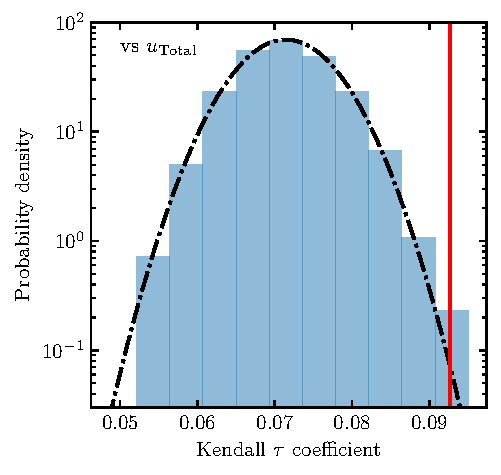
\includegraphics[width=\columnwidth]{Figures/Globular/hist_urad.pdf}
    \caption{ Probability density distribution of the Kendall $\tau$ coefficients for the $L_\gamma$--$u_\mathrm{Total}$ data set. The blue histogram %is from the
    corresponds to the density of the Kendall $\tau$ coefficients of the null hypothesis samples. The dash-dotted line shows the best-fit normally-distributed probability density function for the null hypothesis. The red vertical line indicates the Kendall $\tau$ coefficient for the %real
    actual data.}
    \label{fig:hist}
\end{figure}

\begin{table}
\centering
\caption{Summary of correlations between $L_\gamma$ and four astrophysical parameters of the GCs. The best-fit parameters $a, $b, and the corresponding variance of $L_\gamma$ are found using the EM algorithm. The significance of the correlations is found by MC simulations with Kendall $\tau$ coefficients.}
\label{tab:correlation}
\begin{tabular}{lcccr}
\hline
 Correlation & $a$ & $b$ & $\sqrt{\text{Variance}}$ & Significance\\
\hline
vs $\Gamma_c$ & 0.39 $\pm$ 0.10 & 32.99 $\pm$ 0.26 & 0.59 $\pm$ 0.08 & 6.4$\sigma$\\
vs $u_{\mathrm{Total}}$ & 0.59 $\pm$ 0.09 & 32.97 $\pm$ 0.19 & 0.47 $\pm$ 0.06 & 3.8$\sigma$\\
vs [Fe/H] & 0.35 $\pm$ 0.14 & 34.18 $\pm$ 0.19 & 0.64 $\pm$ 0.08 & 1.8$\sigma$\\
vs $u_\mathrm{MW}$ & 0.29 $\pm$ 0.26 & 33.75 $\pm$ 0.12 & 0.68 $\pm$ 0.09 & 1.5$\sigma$\\
\hline
\end{tabular}
\end{table}

\subsection{Correlation results}

The top (bottom) panel of Figure~\ref{fig:correlation_urad} shows the correlations between $L_\gamma$ and $u_\mathrm{MW}$ ($u_\mathrm{Total}$). GCs with measured $\gamma$-ray luminosity are shown in red, while GCs with upper limits are shown in blue. We find a very small slope for the $L_\gamma$-$u_\mathrm{MW}$ correlation, with $a=0.29 \pm 0.26$, which is almost consistent with 0 considering the large statistical error. The significance of the $L_\gamma$-$u_\mathrm{MW}$ correlation is found to be 1.5$\sigma$. When the total photon field is considered, we find a $L_\gamma$--$u_\mathrm{Total}$ correlation with $a = 0.59 \pm 0.09$. In this case, the significance increases to 3.8$\sigma$. The $L_\gamma$--$u_\mathrm{Total}$ correlation is mostly driven by $u_\mathrm{GC}$, the photon field from the starlight in the GCs (see equation~(\ref{eq:GCRF})). As shown by~Table~\ref{tab:pars}, $u_\mathrm{Total}$ is much greater than $u_\mathrm{MW}$ due to the dominant contribution from $u_\mathrm{GC}$. 

\begin{figure}
    \centering
    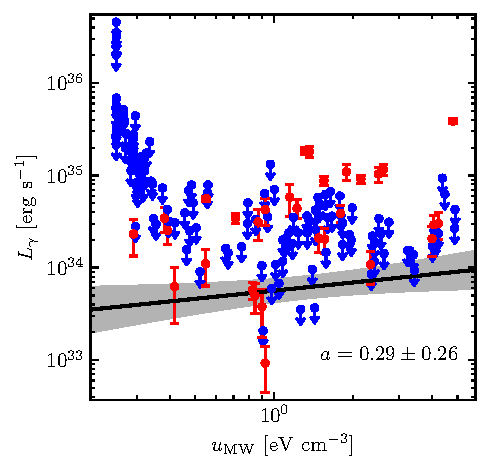
\includegraphics[width=\columnwidth]{Figures/Globular/correlation/L_gamma_vs_isrf_urad.pdf}
    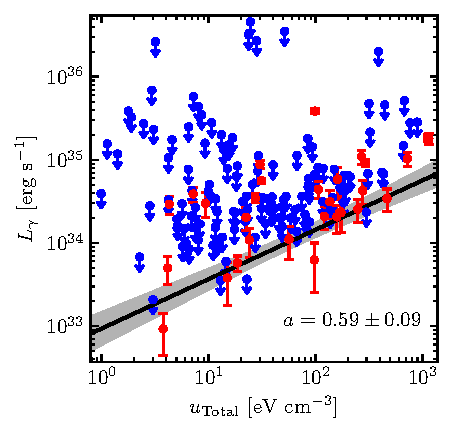
\includegraphics[width=\columnwidth]{Figures/Globular/correlation/L_gamma_vs_total_urad.pdf}
    \caption{\label{fig:correlation_urad} Correlations between $L_\gamma$ and the photon field energy densities. The top panel shows the $L_\gamma$- $u_\mathrm{MW}$ correlation and the bottom panel shows the $L_\gamma$- $u_\mathrm{Total}$ correlation. GCs with measured $\gamma$ rays are shown in red, while GCs with upper limits are shown in blue. The best-fit correlations (black solid lines) are calculated using the EM algorithm discussed in Section~\ref{sec:EM}, with 1$\sigma$ uncertainties included as the gray shaded bands. We find a shallow correlation between $L_\gamma$ and $u_\mathrm{MW}$ with $a = 0.29 \pm 0.26$. The correlation between $L_\gamma$ and $u_\mathrm{Total}$ is more significant, with $a = 0.59 \pm 0.09$. Numerical values of correlations are summarized in Table~\ref{tab:correlation}, along with their significance.
    }
\end{figure}

We also investigate the correlation of the $L_\gamma$'s with the stellar encounter rate ($\Gamma_c$) and GC metallicities ([Fe/H]). These observables are argued to berelated to the formation of MSPs and may provide a proxy for the total number of MSPs in GCs. Figure~\ref{fig:correlation_other} shows the $L_\gamma$--$\Gamma_c$ correlation (top panel) and the $L_\gamma$--[Fe/H] correlation (bottom pannel) obtained with the EM algorithm. We find a positive correlation between the $L_\gamma$ and $\Gamma_c$, with $a = 0.39 \pm 0.10$, for which the Kendall $\tau$ test yields a 6.4$\sigma$ statistical significance. Similarly, we find a correlation between $L_\gamma$ and [Fe/H] with the best-fit value $a = 0.35 \pm 0.14$. However, the statistical significance of the correlation is only 1.8$\sigma$. 

\begin{figure}
    \centering
    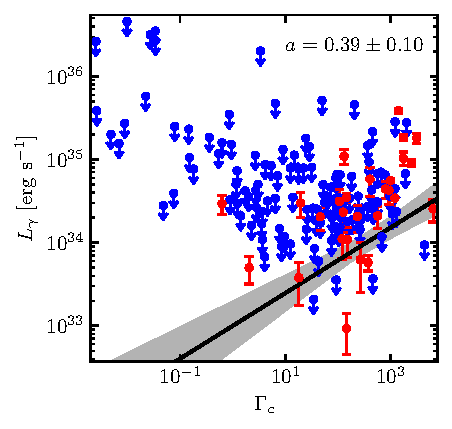
\includegraphics[width=\columnwidth]{Figures/Globular/correlation/L_gamma_vs_encounter_rate.pdf}
    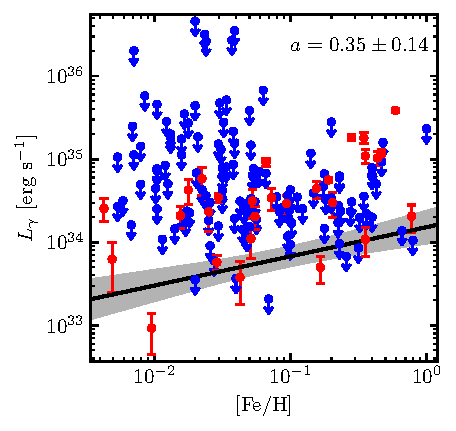
\includegraphics[width=\columnwidth]{Figures/Globular/correlation/L_gamma_vs_metallicity.pdf}
    \caption{\label{fig:correlation_other} Same as Figure~\ref{fig:correlation_urad}, but correlated with the encounter rate (top panel) and metallicity (bottom panel).}
\end{figure}

We summarize the best-fit correlation results and their respective statistical significance in Table~\ref{tab:correlation}.

\subsection{Hidden correlation and interpretations}\label{sec:hidden}

Positive and statistically significant correlations are obtained in both the $L_\gamma$--$u_\mathrm{Total}$ and the $L_\gamma$--$\Gamma_c$ space. The positive $L_\gamma$--$u_\mathrm{Total}$ correlation could indicate a  significant contribution from IC emission. If the $e^\pm$ injected by MSPs lose energy through multiple comparable processes, e.g., IC and synchrotron radiaton, the $L_\gamma$ is proportional to the IC energy loss rates, which is linearly proportional to the $u_\mathrm{Total}$. In the extreme limit where all the $e^\pm$ injected by MSPs lose their energy through IC, the $L_\gamma$ is constrained by the energy injection rate of $e^\pm$ by MSPs and the $u_\mathrm{Total}$ would have less impact. Since we find a preference for a non-linear correlation ($a= 0.59 \pm 0.09$), the $\gamma$ rays are unlikely all originated from IC radiation.

However, the positive correlation between $L_\gamma$ and $u_\mathrm{Total}$ could alternatively be driven by the $L_\gamma$--$\Gamma_c$ correlation. Here, we investigate a potential hidden correlation between $u_\mathrm{Total}$ and $\Gamma_c$ in order to better understand the nature of our detections. Figure~\ref{fig:hidden_0} shows the $u_\mathrm{Total}$ and $\Gamma_c$ values for our sample of GCs. It is apparent that the $u_\mathrm{Total}$ tends to be higher for GCs with higher encounter rates. Since these data are uncensored, we simply estimate the correlation using the Spearman coefficient: we find 0.72, confirming a strong correlation. This result is not surprising because a higher photon density implies higher stellar density which implies higher encounter rates (see also equation~(\ref{eq:encounter})).

\begin{figure}
    \centering
    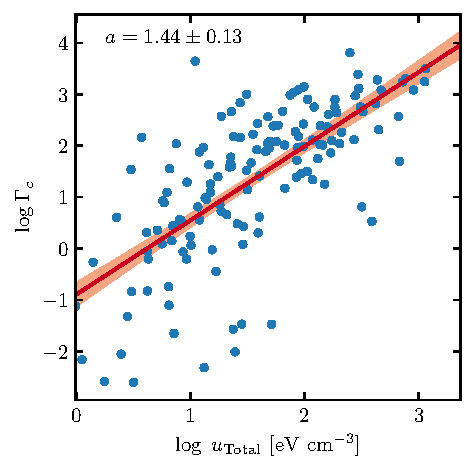
\includegraphics[width=\columnwidth]{Figures/Globular/hidden.pdf}
    \caption{Hidden correlation between $u_\mathrm{Total}$ and $\Gamma_c$. GCs with higher encounter rates tend to have higher total photon field energy densities. The red line shows the relation between $u_\mathrm{Total}$ and $\Gamma_c$ based on a least-squires method in logarithmic space.}
    \label{fig:hidden_0}
\end{figure}

An important implication of this result is that the $L_\gamma$--$u_\mathrm{Total}$ and the $L_\gamma$--$\Gamma_c$ correlations are not necessarily independent. Using a simple least squares method in the logarithmic space, we find the relation between $\Gamma_c$ and $u_\mathrm{Total}$ to be
\begin{equation}
    \Gamma_c \propto u_\mathrm{Total}^{1.44 \pm 0.13}.
\end{equation}
As reported in Table~\ref{tab:correlation}, the correlation between $L_\gamma$ and $\Gamma_c$ has a power index $a=0.39 \pm 0.10$. Based on the hidden relation between $\Gamma_c$ and $u_\mathrm{Total}$, the projected correlation between $L_\gamma$ and $u_\mathrm{Total}$ would have an index $a = 0.56 \pm 0.15$. Within the uncertainty, this projected result is consistent with the directly measured correlation between $L_\gamma$ and $u_\mathrm{Total}$ found in real data, $a = 0.59 \pm 0.09$. Therefore, the positive correlation between $L_\gamma$ and $u_\mathrm{Total}$ could be evidence for IC, or alternatively, an indirect effect of the $L_\gamma$--$\Gamma_c$ correlation which is connected to the dynamic formation of MSPs. The correlation found between $L_\gamma$ and $u_\mathrm{Total}$ cannot be considered as concrete evidence for IC due to this ambiguity implicated by the hidden correlation. However, as we discuss next, evidence for IC emission in GCs may still be revealed from the detailed spectral properties of these objects.

\section{Spectral analysis}\label{sec:spectra}

Motivated by the correlations detected in the previous section, we perform a spectral analysis of the 30 GCs detected in the 4FGL catalog, with the aim of finding further evidence for IC emission. First, we model the spectra of the GCs individually and compare their spectral parameters with those describing the field MSPs. Second, we fit the GCs spectra with universal spectral models which phenomenologically describe possible IC emission. Lastly, we use the detected IC component to constrain the $e^\pm$ injection efficiency in the GCs.

\subsection{Individual spectral fits}\label{sec:spectra_individual}

We consider two possible mechanisms of $\gamma$-ray emission, not mutually exclusive: CR, and IC up-scattering of starlight.

Detailed theoretical models predict that the maximum energy of the $e^\pm$ accelerated by the MSPs is limited by the CR in the pulsar magnetosphere. The predicted CR spectrum exhibits an energy cut-off which is related to the $e^\pm$ Lorentz factor~\citep{2005ApJ...622..531H}. For this reason, we model the GC $\gamma$-ray spectrum--as predicted by CR models--using a power law with an exponential cut-off (PLE) of the form:
\begin{equation}\label{eq:PLE}
    \left[ \frac{dN}{dE} \right]_{\mathrm{CR}} = N_0 \left(\frac{E}{E_0} \right)^{-\Gamma}\exp{ \left( -\frac{E}{E_\text{cut}} \right) },
\end{equation}
where $N_0$ is the normalization factor, $\Gamma$ is the spectral index, $E_0$ is the scaling energy, and $E_\mathrm{cut}$ is the energy cutoff. 

The $e^\pm$ may also leave the MSPs through open magnetic field lines and diffuse into the GC medium. Escaping pairs may up-scatter ambient photons and produce IC emission. The spectrum of the IC is determined by the $e^\pm$ spectrum and the ambient photon field. Theoretical studies~\citep{2011ApJ...743..181H} show that the MSPs can inject $e^\pm$ with Lorentz factors $\gamma_{e^\pm}$ $>$ 10$^6$ efficiently. Given ambient photons of $ E_0\sim$ 1 eV energy, the up-scattered IC photons can reach to above $\gamma_{e^\pm}^2 E_0 = 1$ TeV. Thus, in the Fermi GeV energy range, we assume a power law (PL) injection distribution for $e^\pm$. In the Thomson regime, the IC spectrum resulting from the interaction of power-law-like $e^\pm$ with ambient photons following a black-body radiation distribution~\citep{1970RvMP...42..237B} is still a power law in $\gamma$-ray energy. We consider this spectral form as a phenomenological description of the IC model. Specifically\footnote{For the maximum $\gamma$-ray energy (hundreds of GeV) and the photon field (starlight) we considered, the IC is in transition from the Thomson regime to the Klein-Nishina regime with the Thomson regime still an adequate approximation.},
\begin{equation}\label{eq:PL}
    \left[ \frac{dN}{dE} \right]_{\mathrm{IC}} = N_0 \left(\frac{E}{E_0} \right)^{-\Gamma}.
\end{equation}

We first estimate the GCs' spectral parameters using a maximum likelihood method. For this, we use the CR model and the IC model separately. We perform a $\chi^2$ test using the bin-by-bin $\gamma$-ray fluxes (9 energy bins from 300 MeV to 500 GeV) of each GC and the CR and IC emission models. Therefore, we define 
\begin{equation}
    \chi^2=\sum_i\frac{(F_\text{data}^i-F_\text{model}^i)^2}{(\Delta F_\text{data}^i)^2+(f_\text{ref}^i F_\text{data}^i)^2},
\end{equation}
where $F_\mathrm{data}^i$ and $\Delta F_\mathrm{data}^i$ are the measured fluxes and flux uncertainties obtained at each independent energy bin,  $F_\mathrm{model}^i$ are the predicted fluxes (either the CR or IC models). We allow all model parameters to be free (i.e., normalization, power-law index, and cut-off energy for CR, and normalization and power-law index for IC). The $f_\text{ref}^i$ values encapsulate the systematic uncertainties on the effective area of the LAT. We follow the values reported in the 4FGL catalog~\citep{2020ApJS..247...33A}, and set $f_\text{ref}$ to 0.05 for the first three energy bins, 0.06 for the fourth bin, and 0.1 for the last five bins.

The significance of the spectral curvature is estimated by computing the difference of the best-fit $\chi^2$ between the IC and the CR models, TS$_\mathrm{curve} = \chi^2_\text{IC} - \chi^2_\text{CR}.$ We apply a 2$\sigma$ threshold to determine the type of spectrum: for GCs with TS$_\mathrm{curve} \ge 4$, their PLE spectra are reported. Otherwise, the power-law spectra are reported. Note that this is a lower threshold than the 4FGL, which requires TS$_\mathrm{curve} \ge 9$ before detection of curvature is claimed. We adopt this low threshold because our analysis removes potentially contaminated photons < 300 MeV. Bins encompassing this low energy range usually generate upper limits in the 4FGL analysis and contribute to the detection of curvature. We find, a posteriori, the 2$\sigma$ threshold adequate in our analysis since our fits generate finite $E_\mathrm{cut}$'s within uncertainties for all GCs with TS$_\mathrm{curve} \ge 4$. For those GCs with TS$_\mathrm{curve} < 4$, the fits only generate lower limits for $E_\mathrm{cut}$. Table~\ref{tab:spectra} summarizes the best-fit parameters of the spectra for 30 $\gamma$-ray-detected GCs, sorted by their TS$_\mathrm{curve}$. The majority prefer curved spectra, with only 5 preferring simple power law spectra. Figure~\ref{fig:spectra_example} shows the spectra for 2 GCs as examples. The top panel shows the spectrum of NGC 6397, which is best fit by a simple power law, while the lower panel shows the spectrum for NGC 6541, which prefers an exponential cut-off at $\sim$ 350 MeV with TS$_\mathrm{curve}=4$. 

\begin{table*}
\centering
\caption{Spectral parameters for 30 $\gamma$-ray-detected GCs from the individual fits, ordered from the least curved to the most curved. For GCs with TS$_\mathrm{curve} <$ 4 (2$\sigma$), the best-fit simple power laws (PL) are reported. For the rest GCs, the power laws with an exponential cutoff (PLE) are reported. }\label{tab:spectra}
\begin{threeparttable}
\begin{tabular}{lccccr}
\hline
Name&$\Gamma$ & $\log\left(\frac{E_\mathrm{cut}}{\mathrm{MeV}}\right)$ & $\chi^2$/d.o.f. & Type\tnote{a} & TS$_\mathrm{curve}$\\
\hline
2MS-GC01 & {2.68$\pm$0.08} & ... & 1.03 & PL & 0 \\
NGC 1904 & {2.89$\pm$0.28} & ... & 0.63 & PL & 0 \\
NGC 6397 & {2.56$\pm$0.20} & ... & 0.36 & PL & 2 \\
NGC 7078 & {2.74$\pm$0.16} & ... & 0.70 & PL & 2 \\
NGC 5904 & {2.53$\pm$0.15} & ... & 0.54 & PL & 2 \\
\hline
NGC 6341 & 0.94$\pm$1.12 & {3.24$\pm$0.38} & 0.74 & PLE & 4 \\
NGC 6541 & 1.64$\pm$0.57 & {3.41$\pm$0.37} & 0.25 & PLE & 4 \\
NGC 6528 & 1.85$\pm$0.54 & {3.68$\pm$0.53} & 1.24 & PLE & 4 \\
GLIMPSE02 & 2.58$\pm$0.16 & {3.94$\pm$0.35} & 2.54 & PLE & 5 \\
NGC 6717 & 1.85$\pm$0.34 & {3.71$\pm$0.30} & 0.09 & PLE & 6 \\
NGC 6218 & 0.00$\pm$1.61 & {3.42$\pm$0.10} & 0.43 & PLE & 7 \\
NGC 6402 & 1.86$\pm$0.38 & {3.73$\pm$0.32} & 0.10 & PLE & 7 \\
NGC 2808 & 1.83$\pm$0.33 & {3.75$\pm$0.31} & 0.11 & PLE & 7 \\
NGC 6139 & 1.94$\pm$0.32 & {3.77$\pm$0.26} & 0.43 & PLE & 7 \\
NGC 6838 & 1.38$\pm$0.65 & {3.27$\pm$0.23} & 0.29 & PLE & 9 \\
NGC 6304 & 0.86$\pm$0.81 & {3.10$\pm$0.28} & 0.74 & PLE & 12 \\
M 80 & 1.60$\pm$0.32 & {3.71$\pm$0.24} & 0.31 & PLE & 14 \\
Terzan 2 & 0.60$\pm$0.59 & {3.40$\pm$0.18} & 1.00 & PLE & 16 \\
NGC 6440 & 1.88$\pm$0.22 & {3.63$\pm$0.19} & 1.07 & PLE & 17 \\
NGC 6441 & 1.83$\pm$0.23 & {3.59$\pm$0.21} & 0.84 & PLE & 17 \\
NGC 6652 & 1.29$\pm$0.42 & {3.29$\pm$0.20} & 0.71 & PLE & 22 \\
NGC 6316 & 1.60$\pm$0.23 & {3.54$\pm$0.14} & 1.16 & PLE & 24 \\
NGC 6752 & 0.83$\pm$0.58 & {2.99$\pm$0.20} & 0.18 & PLE & 28 \\
Terzan 1 & 0.00$\pm$0.36 & {3.28$\pm$0.06} & 0.77 & PLE & 37 \\
GLIMPSE01 & 1.67$\pm$0.14 & {3.57$\pm$0.10} & 0.53 & PLE & 61 \\
M 62 & 1.48$\pm$0.14 & {3.47$\pm$0.08} & 0.74 & PLE & 90 \\
Omega Cen & 1.05$\pm$0.27 & {3.25$\pm$0.12} & 1.11 & PLE & 103 \\
NGC 6388 & 1.33$\pm$0.15 & {3.35$\pm$0.07} & 0.46 & PLE & 137 \\
Terzan 5 & 1.58$\pm$0.09 & {3.54$\pm$0.06} & 2.14 & PLE & 159 \\
NGC 104 & 1.28$\pm$0.11 & {3.37$\pm$0.05} & 0.54 & PLE & 207 \\
\hline
\end{tabular}
\begin{tablenotes}
\item [a] Spectrum type: PL for power law; PLE for power law with an exponential cut-off.
\end{tablenotes}
\end{threeparttable}
\end{table*}

\begin{figure}
    \centering
    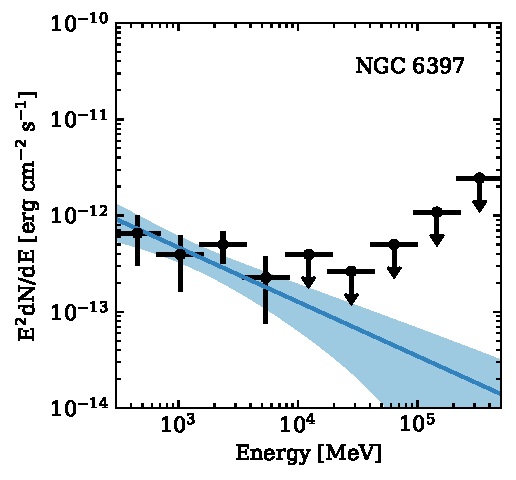
\includegraphics[width=1\columnwidth]{Figures/Globular/spectra/PL_spectrum_16.pdf}
    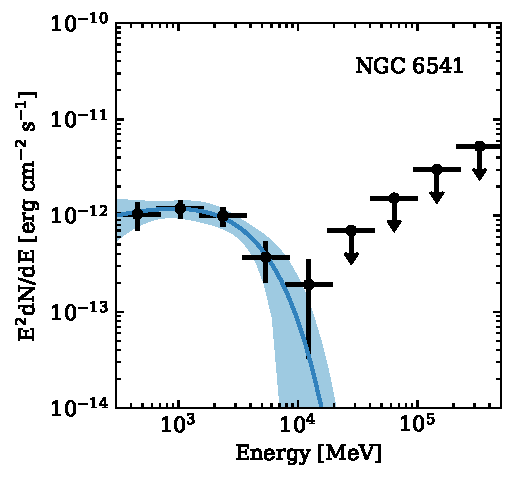
\includegraphics[width=1\columnwidth]{Figures/Globular/spectra/PLE_spectrum_21.pdf}
    \caption{Best-fit spectra (blue solid line) and the 1$\sigma$ uncertainties (blue band) for two GCs. The bin-by-bin fluxes from the Fermi data analysis are included as black points. The top panel shows the spectrum of NGC 6397 as a simple power law because the PLE model is only slightly favored (TS$_\mathrm{curve} = 2$). The bottom panel shows the spectrum for NGC 6541, which prefers an exponential cutoff $\sim$ GeV with TS$_\mathrm{curve} = 4$.}
    \label{fig:spectra_example}
\end{figure}

The \textit{Fermi}-LAT has detected more than 200 pulsars. Most of these have been found to have a curved spectrum with best-fit energy cutoffs of the order of a few GeV. Therefore, their $\gamma$-ray emission is likely dominated by a CR process. {Nevertheless,~\citet{2018PhRvD..98d3005H,2021arXiv210400014H} find} that many MSPs could be surrounded by TeV halos of IC. The IC emission may also extend to the GeV energy range. Figure~\ref{fig:msps} compares the distribution of the spectral parameters of 108 field MSPs in the 4FGL (red dots) with the $\gamma$-ray GCs (blue dots), assuming a PLE spectra. The 1$\sigma$ uncertainties of the best-fit parameters are also shown. We find that within uncertainties, the spectral distribution of the GCs and the field MSPs are very similar. However, given the starlight in GCs typically contributes a much larger photon field energy density than for field MSPs, IC emission may still provide a sizeable contribution to the overall GC $\gamma$-ray emission. The results from individual spectral fit cannot rule out the presence of IC for the following reasons: (1) There are 5 GCs for which the spectra shows no obvious energy cutoffs. This is hard to explain using the CR emission model alone. (2) Many GCs have energy bins above 10 GeV detected even though their spectra have cutoffs of order a GeV (see Appendix~\ref{appx:spectra}). These high-energy measurements may be indicative of an IC component.

\begin{figure}
    \centering
    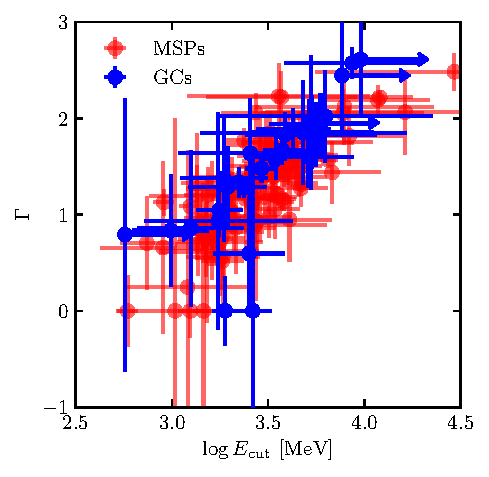
\includegraphics[width=\columnwidth]{Figures/Globular/msp_vs_gc.pdf}
    \caption{Spectral parameters of the $\gamma$-ray emission. The PLE spectrum is assumed, with $\Gamma$ and $E_\mathrm{cut}$ as free parameters. Both the GCs (blue dots) and the MSPs (red dots) detected in the 4FGL are included. The error bars represent the 1$\sigma$ parameter uncertainties. Within uncertainties, the distribution of the GCs' spectra is very similar to that of the MSPs.}
    \label{fig:msps}
\end{figure}

\subsection{Fit assuming universal spectral components}\label{sec:spectra_global}

The curvature of the GCs' spectra at around a few GeV's, as well as their similarity to the field MSPs spectra, support the hypothesis that the GeV $\gamma$-ray emission from most GCs is due to mainly local CR emission from MSPs within GCs. However, IC may still contribute sub-dominantly, especially at the high-energy end. To probe this possibility, we perform a reduced $\chi^2$ analysis in which we fit, bin-by-bin, the  GCs' spectra using a linear combination of the spectral components introduced in equation~\ref{eq:PLE} and \ref{eq:PL}. Specifically;
\begin{align}\label{eq:PLE+PL}
    \frac{dN}{dE} &= \left[ \frac{dN}{dE} \right]_\mathrm{CR} + \left[ \frac{dN}{dE} \right]_\mathrm{IC} \\\nonumber
    &= N_1\left( \frac{E}{E_0} \right)^{-\Gamma_1}\exp\left(-\frac{E}{E_\mathrm{cut}}\right) + N_2\left(\frac{E}{E_0}\right)^{-\Gamma_2}.
\end{align}

Fitting such a two-component model to each GC's bin-by-bin data is difficult since the GC spectra only contains 9 energy bins, and many high energy bins only provide upper limits. On the other hand, typical GCs can host close to $\sim$ 20 MSPs~\citep{2019ApJ...877..122Y} each. So, as a simplifying approximation, we hypothesise that the $\gamma$-ray and $e^\pm$ injection from the collection of MSPs in each GC to be similar to one another. Then, we can fit a common or universal spectrum to all the $\gamma$-ray detected GCs, i.e., one set of spectral shape parameters in the two component model in equation~(\ref{eq:PLE+PL}) for all the GCs. More specifically, we tie the $\Gamma_1$, $\Gamma_2$ and $E_\mathrm{cut}$ across all GCs considered (hereafter referred to as the ``universal model''). The normalization factors $N_1$ and $N_2$ are allowed to float for each GC as these should depend on the number of MSPs and the photon field energy density in the GCs.

We perform the universal fit by minimizing the total $\chi^2$ of 30 $\gamma$-ray-detected GCs,
\begin{equation}
    \chi^2_\mathrm{total}(\Gamma_1,\;\Gamma_2,\;E_\mathrm{cut}) = \sum_i\chi_i^2(\Gamma_1,\;\Gamma_2,\;E_\mathrm{cut},\;N_1^i,\;N_2^i).
\end{equation}
In practice, we assign the same $\Gamma_1$, $\Gamma_2$, and $E_\mathrm{cut}$ to all $\gamma$-ray GCs and perform a minimum $\chi^2$ for each different object. However, during the fit, we free the $N_1^i$ and $N_2^i$ parameters. By scanning the parameter space of $\Gamma_1$, $\Gamma_2$, and $E_\mathrm{cut}$, we find the values that minimize the total $\chi^2$ for the two-component model. These are, 
\begin{align}\nonumber
    \Gamma_1 = 0.88 \pm 0.44,\\\nonumber
    \Gamma_2 = 2.79 \pm 0.25,\\\nonumber
    \log\left(\frac{E_\mathrm{cut}}{\mathrm{MeV}}\right) = 3.28 \pm 0.16,
\end{align}
for which we find a $\chi^2_\mathrm{total} / \mathrm{d.o.f} = 204/206 = 0.99$ (we have $30\times 9$ data points, and the number of free parameters is $60+3$ as there are 2 normalization factors for each GC, and 3 global parameters. So, we have $\mathrm{d.o.f}=30\times 9 - 60 - 3 -1 = 206$). In Figure~\ref{fig:global}, we show the associated 3$\sigma$ contours and correlated uncertainties for the parameters $\Gamma_1$, $\Gamma_2$, and $E_\mathrm{cut}$ as found in this procedure.

\begin{figure*}
    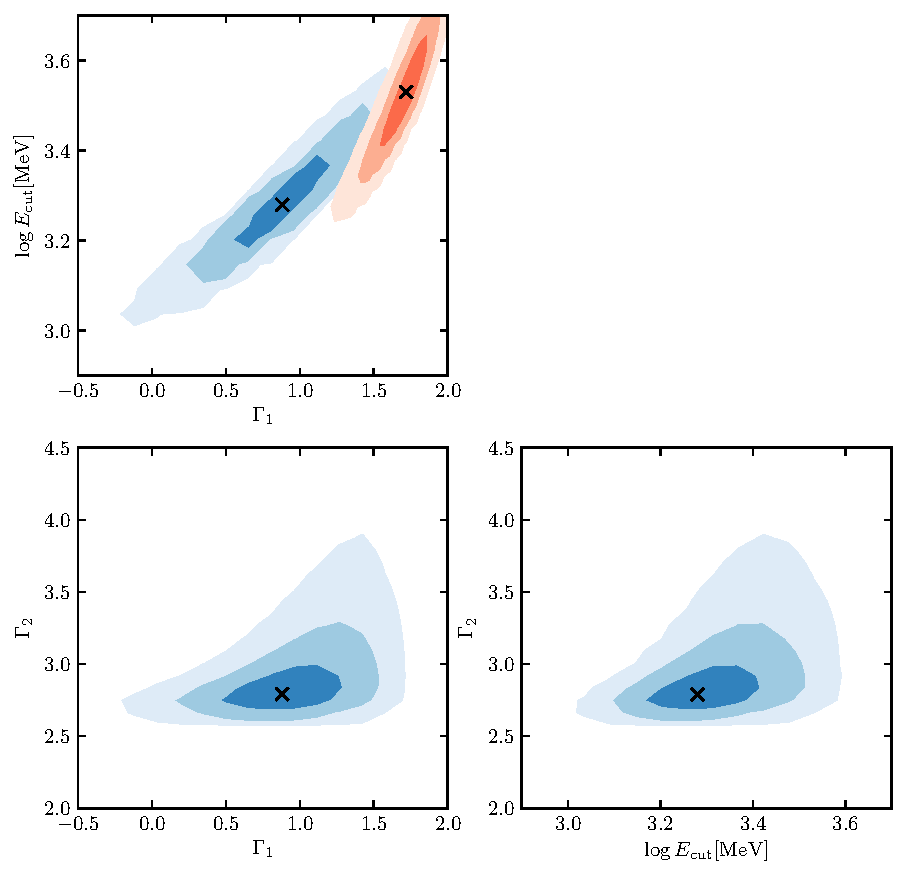
\includegraphics[width=0.8\textwidth]{Figures/Globular/globalfit.pdf}
    \caption{The projected parameter space of the universal model fit, as illustrated in equation~(\ref{eq:PLE+PL}). The blue shaded contours show the 1$\sigma$, 2$\sigma$, and 3$\sigma$ confidence levels for the two-component model. The crosses indicate the best fit values for $\Gamma_1$, $\Gamma_2$, and $E_\mathrm{cut}$. On the top-left panel, the red shaded region shows the best-fit value and 3$\sigma$ confidence levels for the null hypothesis, which includes only the CR model.}
    \label{fig:global}
\end{figure*}

In order to compute the statistical significance of the {PL} component, it is necessary to define the null hypothesis. This corresponds to the universal model containing only the CR component (see equation~\ref{eq:PLE}). Again, we tie $\Gamma_1$ and $E_\mathrm{cut}$ across all GCs and allow the normalization factors to individually vary. We find that the best-fit parameters for the CR-only model are:
\begin{align}\nonumber
    \Gamma_1 = 1.72 \pm 0.21, \\\nonumber
    \log\left(\frac{E_\mathrm{cut}}{\mathrm{MeV}}\right) = 3.53 \pm 0.19.
\end{align}
In this case, we find a $\chi^2_\mathrm{total} / \mathrm{d.o.f} = 349/237=1.47$ (the null hypothesis has 30 + 2 free parameters so the $\mathrm{d.o.f}=30\times 9 - 30 - 2 - 1 = 237$). This implies that the two-component model is preferred at the 8.2$\sigma$ level ($\Delta \chi^2=349-204$ for 31 d.o.f [1 power-law index plus 30 normalization factors]). It is useful to compare the best-fit spectral results of the CR component for the universal models with the best-fit spectral parameters of the MSPs in the 4FGL catalog. As seen in Figure~\ref{fig:msps_global}, although the CR-only model (null hypothesis) has larger $\Gamma$ and higher $E_\mathrm{cut}$ than the CR component from the two-component model, our results for both models are compatible with the field MSPs, up to statistical uncertainties.

The universal fitting procedure used in this section is similar to a stacking analysis. This method is usually applied to explore the characteristics of an astrophysical population, especially one that is undetected. Numerous studies have shown that this technique can increase the detection sensitivity to such population characteristics. So, even though there is good statistical evidence for the {PL} component in the universal fit,  this might not be apparent from individual fitting of the two-component model.

We show examples of the spectra obtained in the universal fit of the two-component model for NGC 6397 and NGC 6541 in Figure~\ref{fig:global_spectra}. As can be seen, the solutions for the CR and {PL} components look physically plausible. The spectra also include 1$\sigma$ bow-tie errors, which immediately reveal the level of statistical support for the CR and {PL} components, respectively. For comparison, the results shown in Figure~\ref{fig:spectra_example} presented a {single-component (e.g.,~\citet{2020ApJS..247...33A})} spectral curvature analysis applied to NGC 6397 and NGC 6541, individually. 

\begin{figure}
    \centering
    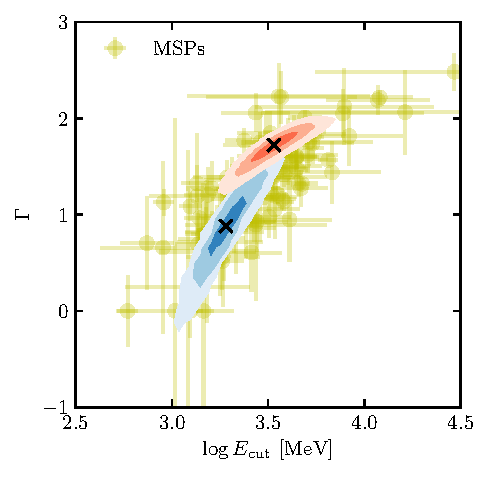
\includegraphics[width=\columnwidth]{Figures/Globular/msp_vs_gc_global.pdf}
    \caption{Same as Figure~\ref{fig:msps}, but with best-fit parameters of GC replaced by those obtained from the universal models. The 3$\sigma$ contours are shown for the CR-only model (red) and the CR component from the two-component model (blue), as in Figure~\ref{fig:global}. The MSP parameters are included in the background (yellow dots).}
    \label{fig:msps_global}
\end{figure}

We show some additional noteworthy results of the universal fit in Figure~\ref{fig:global_spectra_ul}. Here, we see that in the case of GC 2MS-GC01, the {PL} model is sufficient to explain the bin-by-bin spectrum over the full energy range, but we also display the estimated 95\% C.L. upper limit for the normalization of the CR model. By contrast, in the case of GC M 80, we find that the data is best described by the CR model alone, and we show the 95\% C.L. upper limit for the normalization of the {PL} component. These examples might indicate special conditions of the environment of the GC.

For 19 GCs (out of the 30 GCs included in the universal fit), we find good statistical support for both the CR and {PL} models. For the remaining 11 GCs we find that only one component is sufficient to explain the spectrum: 7 GCs require only the CR model and the other 4 GCs require only the {PL} model. The two-component spectral results for all 30 GCs are shown in Appendix~\ref{appx:spectra}.

To explain the best-fit index of the {PL} component ($\Gamma_2 = 2.79 \pm 0.25$) {as IC emission}, the implied emitting $e^\pm$ spectrum would have an index of $4.58 \pm 0.50$. The minimum $e^\pm$ energy required to maintain a power law IC in the energy range of our analysis (300 MeV) is $\lesssim$ 10 GeV given that the upscattered photon field has energies $\sim$ 1 eV~\citep{1970RvMP...42..237B}. Interestingly,~\citet{2011ApJ...743..181H} has simulated $e^{\pm}$ pair cascades from pulsar polar caps. For typical MSP parameters, they show that the injected $e^\pm$ flux decreases by $\sim 5 - 10$ orders of magnitude when the $e^\pm$ energy increases from $\sim$10 GeV to $\sim$ 1 TeV. The soft $e^\pm$ spectrum we found is in line with their results.

\begin{figure}
    \centering
    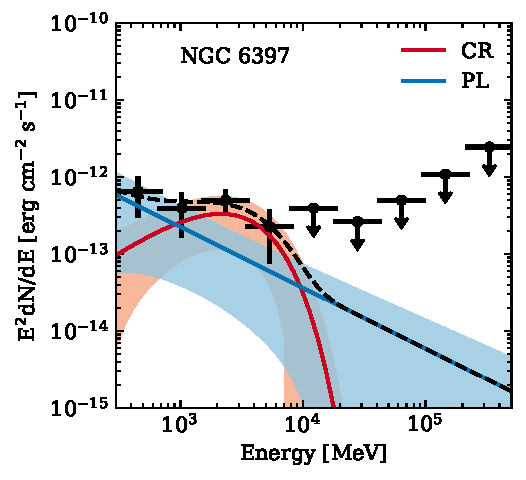
\includegraphics[width=1\columnwidth]{Figures/Globular/spectra/2comp_16.pdf}
    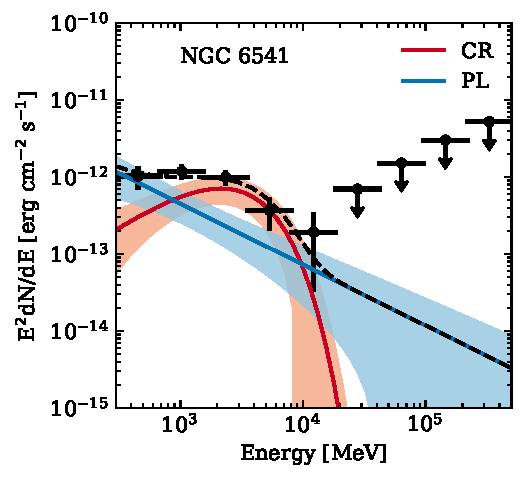
\includegraphics[width=1\columnwidth]{Figures/Globular/spectra/2comp_21.pdf}
    \caption{The best-fit two-component spectra for NGC 6397 (top panel) and NGC 6541 (bottom panel). The spectra are fit to a universal shape with same $\Gamma_1$, $\Gamma_2$, and $E_\mathrm{cut}$ for all GCs.  Only the normalizations of the two components are allowed to vary between GCs. The best-fit parameters for the CR component (red line with shaded band) is $\Gamma_1 = 0.88 \pm 0.44$ and $\log(E_\mathrm{cut}/\mathrm{MeV})=3.28 \pm 0.16$. The best fit parameter for the {PL} component (blue line with shaded band) is $\Gamma_2 = 2.79 \pm 0.25$. The black dashed line indicates the total of the two components.}
    \label{fig:global_spectra}
\end{figure}

\begin{figure}
    \centering
    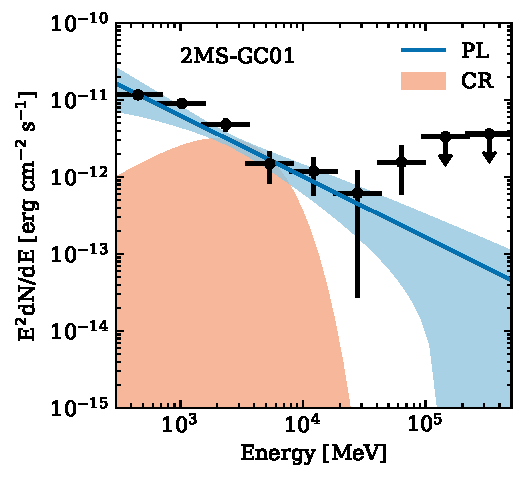
\includegraphics[width=1\columnwidth]{Figures/Globular/spectra/2comp_0.pdf}
    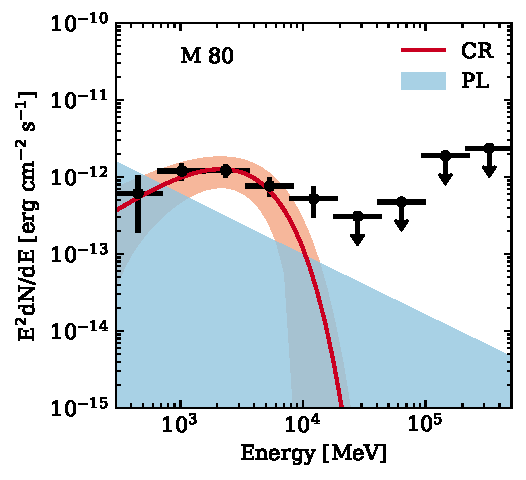
\includegraphics[width=1\columnwidth]{Figures/Globular/spectra/2comp_8.pdf}
    \caption{Spectra of 2MS-GC01 (top panel) and M 80 (bottom panel) from the two-component fit. The 2MS-GC01 prefers only the {PL} model (blue solid line). The 95\% upper limit on the normalization of the CR model is shown by the red shaded region. In contrast, only the CR model is detected for M 80 (red solid curve). The 95\% upper limit on the normalization of the {PL} model is shown by the blue shaded region.}
    \label{fig:global_spectra_ul}
\end{figure}

\subsection{Leptonic injection efficiency within the globular clusters}\label{spectra_fe}

The relative normalization of the CR and IC components probes an important property of the MSPs: the $\gamma$-ray production and $e^\pm$ injection efficiencies, respectively. Indeed, the spin-down energy of MSPs can be injected into $\gamma$ rays and $e^\pm$. While prompt $\gamma$ rays are mainly produced by CR in the magnetosphere, the $e^\pm$ can propagate into the interstellar environment. We can write down the following empirical relations,
\begin{align}
    L_\mathrm{CR} &= f_\gamma L_\mathrm{sd},\\
    L_{e^\pm} &= f_{e^\pm} L_\mathrm{sd},
\end{align}
where $L_\mathrm{sd}$ is the spin-down luminosity and the $f$'s are efficiency parameters. 

Assuming that the $\gamma$-ray emission is the superposition of CR and IC processes, we have that
\begin{equation}
    L_\gamma = L_\mathrm{CR} + L_\mathrm{IC}.
\end{equation}
However, $e^\pm$ can also lose energy via synchrotron radiation. We can compare the relative strength of the sychrotron radiation vs the IC emission through
\begin{equation}
    \frac{\dot{E}_\mathrm{SR}}{\dot{E}_\mathrm{IC}} = \frac{u_\mathrm{B}^2}{u_\mathrm{rad}^2},
\end{equation}
where $\dot{E}_\mathrm{SR}$ and $\dot{E}_\mathrm{IC}$ are the synchrotron and IC energy loss rates, respectively, $u_\mathrm{B}$ is the magnetic energy density, and $u_\mathrm{rad}$ is the radiation field energy density. We note that this relation assumes that the $e^\pm$ lose all their energy within the GCs. We provide justifications for this assumption in Appendix~\ref{appx:system_fe}. For a typical GC the magnetic field is estimated to be $B\lesssim \mathrm{10\;\mu G}$~\citep{2007MNRAS.377..920B}, so we expect to have a $u_\mathrm{B} = {\mathrm{(10\;\mu G)}^2}/{(2\mu_0)} = 2.5$ eV cm$^{-3}$, which is much smaller than the total radiation field of most GCs shown in Table~\ref{tab:pars}. Thus in the usual instance when IC is the leading energy loss process, we have that
\begin{equation}
    L_\mathrm{IC} \simeq L_{e^\pm}.
\end{equation}

Since no GC is detected as an extended source by the \textit{Fermi}-LAT, the energy carried away to the interstellar medium by $e^\pm$ propagation is expected to be small. Thus, we can use the following approximate scaling relation,
\begin{equation}\label{eq:fefgamma}
    \dfrac{f_{e^\pm}}{f_\gamma} \simeq \dfrac{L_\mathrm{IC}}{L_\mathrm{CR}}.
\end{equation}
Using this\footnote{We discuss caveats to the approximation used in equation~(\ref{eq:fefgamma}) in Appendix~\ref{appx:system_fe}.}, we estimate the ratios $f_{e^\pm}/f_\gamma$ for all $\gamma$-ray emitting GCs in Table~\ref{tab:ratio}. These are found to be in the range $\approx 0.17 - 1.04$. Note that for some GCs we present only upper or lower limits as only one component is detected. The measurement of pulsars by \textit{Fermi}-LAT estimated the $f_{\gamma}$ efficiency from observations of pulsars and found that on average, $f_\gamma \sim \mathrm{10\%}$. Furthermore, the $e^\pm$ efficiency $f_{e^\pm}$ was also estimated to be around 10\% from TeV observations of {nearby pulsars~\citep{2017PhRvD..96j3013H, 2018PhRvD..98d3005H, 2021arXiv210400014H} and} the Galactic center~\citep{2013MNRAS.435L..14B}, although \citet{2019MNRAS.484.2876M} claims $f_{e^\pm}$ is at the percentage level for one GC they observed (NGC 7078), and \citet{2020arXiv200508982S} suggest $f_{e^\pm} \sim 90\%$ on the basis of the  radio continuum emission detected from galaxies with low specific star formation rates.

For the CR and IC luminosities, we integrate the best-fit two-component spectra from 300 MeV to 500 GeV, the same energy range used in the Fermi data analysis. For the IC emission, the minimum $e^\pm$ injection energy probed by this energy range is $\lesssim$ 10 GeV assuming the ambient photon field is starlight. We note that \citet{2011ApJ...743..181H} investigated the $e^\pm$ pair cascades from MSPs and proposed several theoretical models. Their Figure 10 shows that their predicted pair spectra peak at $\sim$ GeV and extend to $\gtrsim$ TeV. This roughly corresponds to the Fermi energy range we assume. If the $e^\pm$ injection spectra extend to lower energy, they will lead to higher $L_\mathrm{IC}$. Therefore, the choice of $\gamma$-ray energy range will contribute as systematic uncertainties on the estimated $f_{e^\pm}/f_\gamma$. For example, we verify that the $f_{e^\pm}/f_\gamma$ would be $\sim$ 5 times larger if the minimum $\gamma$-ray energy is assumed to be 30 MeV.

\begin{table}
    \centering
    \caption{$\gamma$-ray luminosity for the IC and CR  components and the ratios between $f_{e^\pm}$ and $f_\gamma$. For GCs with only one component detected, the 95\% C.L. upper limits are reported for another component.}
    \begin{tabular}{lccr}
\hline
Name & $L_\mathrm{{IC}}$ & $L_\mathrm{CR}$ & $f_{e^\pm}/f_\gamma$ \\
 & (10$^{34}$ erg s$^{-1}$) & (10$^{34}$ erg s$^{-1}$) &  \\
\hline
GLIMPSE02 & 10.90 $\pm$ 1.06 & < 1.70 & > 6.40 \\
2MS-GC01 & 3.20 $\pm$ 0.44 & < 1.08 & > 2.95 \\
NGC 7078 & 2.38 $\pm$ 0.62 & < 1.14 & > 2.08 \\
NGC 1904 & 1.75 $\pm$ 0.75 & < 1.62 & > 1.08 \\
NGC 5904 & 0.54 $\pm$ 0.31 & 0.52 $\pm$ 0.24 & 1.04 $\pm$ 0.77 \\
NGC 6397 & 0.05 $\pm$ 0.04 & 0.05 $\pm$ 0.03 & 0.97 $\pm$ 1.00 \\
NGC 6440 & 4.83 $\pm$ 1.20 & 5.12 $\pm$ 0.97 & 0.94 $\pm$ 0.29 \\
NGC 6541 & 0.99 $\pm$ 0.42 & 1.09 $\pm$ 0.35 & 0.92 $\pm$ 0.48 \\
NGC 6139 & 2.33 $\pm$ 1.14 & 2.64 $\pm$ 0.90 & 0.88 $\pm$ 0.52 \\
NGC 6441 & 8.36 $\pm$ 1.80 & 9.57 $\pm$ 1.57 & 0.87 $\pm$ 0.24 \\
NGC 6752 & 0.25 $\pm$ 0.09 & 0.33 $\pm$ 0.08 & 0.76 $\pm$ 0.33 \\
NGC 6717 & 0.80 $\pm$ 0.42 & 1.19 $\pm$ 0.35 & 0.67 $\pm$ 0.40 \\
NGC 6402 & 1.18 $\pm$ 0.79 & 1.83 $\pm$ 0.62 & 0.65 $\pm$ 0.48 \\
NGC 2808 & 1.18 $\pm$ 0.63 & 2.09 $\pm$ 0.56 & 0.56 $\pm$ 0.34 \\
NGC 6838 & 0.16 $\pm$ 0.14 & 0.28 $\pm$ 0.11 & 0.55 $\pm$ 0.54 \\
GLIMPSE01 & 2.77 $\pm$ 0.65 & 5.89 $\pm$ 0.62 & 0.47 $\pm$ 0.12 \\
NGC 6316 & 2.99 $\pm$ 1.44 & 7.71 $\pm$ 1.26 & 0.39 $\pm$ 0.20 \\
Terzan 5 & 10.02 $\pm$ 1.68 & 27.46 $\pm$ 1.83 & 0.37 $\pm$ 0.07 \\
NGC 6652 & 1.16 $\pm$ 0.77 & 3.35 $\pm$ 0.68 & 0.35 $\pm$ 0.24 \\
M 62 & 2.20 $\pm$ 0.60 & 6.92 $\pm$ 0.63 & 0.32 $\pm$ 0.09 \\
NGC 6388 & 4.37 $\pm$ 1.18 & 14.22 $\pm$ 1.27 & 0.31 $\pm$ 0.09 \\
NGC 104 & 0.96 $\pm$ 0.22 & 4.67 $\pm$ 0.30 & 0.21 $\pm$ 0.05 \\
Omega Cen & 0.50 $\pm$ 0.24 & 2.90 $\pm$ 0.27 & 0.17 $\pm$ 0.08 \\
NGC 6528 & < 2.41 & 1.38 $\pm$ 0.58 & < 1.74 \\
NGC 6218 & < 0.39  &  0.23 $\pm$ 0.12 & < 1.67 \\
NGC 6341 & < 0.71  &  0.49 $\pm$ 0.23 & < 1.45 \\
NGC 6304 & < 0.79  &  0.89 $\pm$ 0.30 & < 0.88 \\
M 80 & < 2.31  &  3.45 $\pm$ 0.74 & < 0.67 \\
Terzan 2 & < 0.49  &  2.66 $\pm$ 0.52 & < 0.18 \\
Terzan 1 & < 0.16  &  2.42 $\pm$ 0.49 & < 0.07 \\
\hline
    \end{tabular}
    \label{tab:ratio}
\end{table}

\section{Discussion}\label{sec:discussion}

\subsection{Implications of the correlation analysis}

We have found strong positive correlations between $L_\gamma$, the stellar encounter rate $\Gamma_c$, and the total photon field energy density $u_\mathrm{Total}$ of GCs. The latter correlation may indicate a significant contribution of IC upscattering of ambient starlight to the total $\gamma$-ray emission of GCs. However, we showed in Figure~\ref{fig:hidden_0} that the $u_\mathrm{Total}$ also increases with $\Gamma_c$. So, the detection of the $L_\gamma$--$u_\mathrm{Total}$ correlation alone does not unambiguously demonstrate the presence of IC emission in GCs~\footnote{We also analyzed other potential hidden correlations, but no obvious correlations with other parameters such as the interstellar radiation field and the distance from the Sun were found (see Appendix~\ref{appx:system_fe}).}. On the other hand, corroborating evidence for IC emission was found from the universal two-component fit, wherein we were able to estimate, separately, the luminosities of the CR and IC components of most GCs. The ratios of the luminosities between the CR and IC components were found to be comparable. This implies that MSPs in GCs can potentially inject $e^{\pm}$ as efficiently as they inject prompt magnetospheric $\gamma$ rays.

Overall, our correlation results in the $L_\gamma$-$\Gamma_c$ plane are consistent with those in \citet{2011ApJ...726..100H} and~\citet{2019MNRAS.486..851D}, though it is important to note that our method is more statistically robust since we include GCs with detection limits which were previously neglected. In particular, our high significance ($6.4\sigma$) detection of a $L_\gamma$--$\Gamma_c$ correlation naively supports a dynamic formation scenario for MSPs in GCs. However, as pointed out earlier, this correlation may not be independent due to the hidden correlation of $u_\mathrm{Total}$ and $\Gamma_c$. On the other hand, we have not found an obvious correlation between $f_{e^\pm}/f_\gamma$ and $u_\mathrm{Total}$ (see Appendix~\ref{appx:system_fe}). The lack of this latter correlation may indicate that IC is, in fact, the leading energy loss process for $e^\pm$ in GCs: in the limit of IC dominance, the IC luminosity of GCs already saturates the power going into freshly-injected $e^\pm$ pairs, so ``dialling-up'' the light field energy density has no effect on the IC luminosity. Thus, in this situation of IC dominance, we expect, at most, only a weak correlation between $L_\gamma$ and $u_\mathrm{Total}$ and we would anticipate that the $L_\gamma$-$\Gamma_c$ correlation is the fundamental one (while the $L_\gamma$-$u_\mathrm{Total}$ correlation is caused by the fact that GCs with higher stellar encounter rate naturally have higher stellar density which leads to higher photon field density). With the uncertainties of the data and the number of variables involved, it is challenging to statistically confirm this scenario. Overall, however, our results are consistent with there being both a significant role for dynamical formation of MSPs in GCs and for the presence of a significant contribution of IC to the overall $\gamma$-ray emission of GCs.

Previous studies~\citep{2011ApJ...726..100H} found a positive correlation between $L_\gamma$ and $u_\mathrm{MW}$, and $L_\gamma$ and [Fe/H]. However, our study does not confirm these results. The former discrepancy is possibly due to the different interstellar radiation field models assumed in these works, or it could be due to the more limited sample data used in~\cite{2011ApJ...726..100H}. Specifically, while we have used the most up-to-date interstellar radiation field for the Milky Way--which is the 3D radiation field model in GALPROP v56~\citep{2017ApJ...846...67P}$-$ ~\citet{2011ApJ...726..100H} used the 2D radiation field model in GALPROP v54. Also, as explained above, our correlation study includes 30 $\gamma$-ray-detected GCs , as well as the luminosity upper limits from the 127 non-detected ones, thus covering the entire GC~\citet{1996AJ....112.1487H} catalog. As for the latter discrepancy, similar results for the $L_\gamma$--[Fe/H] correlation were obtained by~\citet{2019MNRAS.486..851D}, which also found low statistical evidence for this correlation.

\subsection{Implications for the Fermi GeV excess}

The emission from a putative population of about $40,000$~\citep{2020JCAP...12..035P} unresolved MSPs in the Galactic Center region is currently the preferred explanation for the Fermi GeV excess~\citep{2018NatAs...2..387M,2018NatAs...2..819B,2019JCAP...09..042M,2020PhRvD.102d3012A}. Since GCs also contain large numbers of unresolved MSPs, it is useful to compare the light-to-mass ratios for these two systems so as to obtain additional clues for the physical processes causing the observed high-energy $\gamma$-ray emissions in their directions. In Figure~\ref{fig:stellar_mass}, we show the relation between $L_\gamma$ and the stellar mass for several different systems. The blue dots show the sample of the $\gamma$-ray detected GCs in this work. The nuclear bulge (orange dot) has a stellar mass around $1.4\times 10^9$ M$_\odot$ and a $\gamma$-ray luminosity of $(3.9\pm 0.5)\times 10^{36}$ erg s$^{-1}$ and the boxy bulge (green dot) has $1.5\times 10^{10}$ M$_\odot$ and $(2.2 \pm 0.4)\times 10^{37}$ erg s$^{-1}$~\citep{2019JCAP...09..042M}. The combination of the nuclear bulge and the boxy bulge is responsible for the Galactic center GeV excess. Also included are the Galactic disk (red dot) luminosity predicted by~\citet{2018NatAs...2..819B} and the M31 galaxy (purple star)~\citep{2017ApJ...836..208A}. The dot-dashed line shows the $\gamma$-ray luminosity-to-stellar-mass relation implied for the nuclear bulge and the boxy bulge, which is $2 \times 10^{27}$ erg s$^{-1}$ M$_\odot^{-1}$. 

As can be seen in Figure~\ref{fig:stellar_mass}, the luminosities of the detected sample of GCs exceed the luminosities expected based on the bulge correlations. In total, the GC samples have a stellar mass of $\sim 1.4\times 10^7$ M$_\odot$ and a $\gamma$-ray luminosity of $\sim 1.5\times 10^{36}$ erg s$^{-1}$. This means that GCs systematically emit $\sim$ 50 times more $\gamma$ rays per stellar mass than other objects such as the nuclear bulge and the Galactic bulge. The GCs have long been known for producing MSPs efficiently~\citep{2005ASPC..328..147C}. On average GCs make up $\sim 0.05\%$ of the total number of stars in the Milky Way~\citep{2019ApJ...877..122Y}, but more than one-third of the known MPSs are found in these systems~\citep{2005AJ....129.1993M}. Our observations support this scenario. This is also consistent with the larger stellar densities and larger stellar encounter rates in GCs than in the Galactic bulge. We also note in passing that a large fraction of $\gamma$-ray-detected GCs are located in the Galactic bulge region (see Figure~\ref{fig:all_sky_distribution}), which means that it is possible that at least some of the unresolved MSPs contributing to the Fermi GeV excess are hosted by GCs in the Galactic bulge region.

\begin{figure}
    \centering
    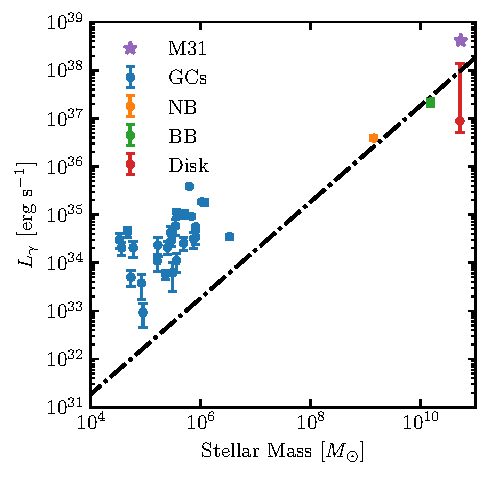
\includegraphics[width=1\columnwidth]{Figures/Globular/mass.pdf}
    \caption{Relations between $L_\gamma$ and the stellar mass for several systems. The results for the nuclear bulge (orange dot) and boxy bulge (green dot) are adopted from~\citet{2019JCAP...09..042M}. The Galactic disk (red dot) luminosity is predicted by~\citet{2018NatAs...2..819B}, and the M31 (purple star) are adopted from~\citet{2017ApJ...836..208A}. The blue dots show the data for 30 $\gamma$-ray detected GCs. The dash-dotted line is the relation implied by the nuclear bulge and boxy bulge.}
    \label{fig:stellar_mass}
\end{figure}

\subsection{TeV observations of globular clusters}

Using the universal two-component fit, we identified a power law component with a slope of $2.79 \pm  0.25$ from the spectra of $\gamma$-ray-detected GCs. The power law component can be plausibly explained by IC emission from GCs. The fact that this power law component is rather soft may explain why most GCs are not detected in the TeV energy range. In order to explore this more closely, we extrapolate the high energy tail of the GCs spectra to TeV energies in Figure~\ref{fig:TeV}. In this figure, the black line shows the extrapolated fluxes for Terzan 5, and the gray band shows the range of extrapolated fluxes for the other 23 GCs with a detected IC component. Above 100 GeV, {\it Fermi}-LAT only find upper limits (blue arrows) for Terzan 5. The red dots are the H.E.S.S. measurements from the direction of Terzan 5. It is interesting to note that the extrapolated spectrum for Terzan 5 is about one order of magnitude lower than the H.E.S.S. measurements from the same object. This discrepancy might be explained by the fact that the $\gamma$-ray source reported by H.E.S.S is misaligned with the center of Terzan 5 so that this association could be a chance coincidence. However, such a coincidence with known objects has been estimated to be improbable ($\sim 10^{-4}$)~\citep{2011A&A...531L..18H}. If the H.E.S.S. source is indeed associated to Terzan 5, it could be that $e^\pm$ injection spectrum from MSPs has a spectral break at approximately 1 TeV. Note that a substantial fraction of stars in Terzan 5 have been identified as young and centrally concentrated~\citep{2016ApJ...828...75F,2020BAAA..61R...90G}, which could lead to a larger number of younger pulsars. The H.E.S.S. measurements could be explained if these young pulsars have higher energy $e^\pm$ cutoffs. Therefore, Terzan 5 may not be representative compared to other GCs which are dominated by old stellar systems. However, \citet{2019AJ....158...14N} also find that the abundance variations among Terzan 5 is indeed consistent with a regular globular cluster. Alternatively, the TeV $\gamma$ rays could originate from sources other than MSPs (e.g., hadronic emission from supernova remnants). Further investigation of those scenarios, though very interesting, is beyond the scope of this work. 

We also include in Figure~\ref{fig:TeV} the sensitivities to point-like sources for the next generation $\gamma$ ray observatories. The green line shows the sensitivity for the Cherenkov Telescope Array (CTA)$-$South assuming 100 hours of observation time. The purple line shows the 1-year sensitivity of the Large High Altitude Air Shower Observatory (LHAASO). The extrapolated IC fluxes are close to the 100-hour CTA sensitivity. It is clear that it will be difficult for the next-generation TeV $\gamma$-ray telescopes to actually detect each individual GC considered in our study. This might require a much more ambitious observation strategy that increases the sensitivity by factor of a few at the TeV energy range.  Efforts to measure the diffuse IC emission from the putative MSP population responsible for the Fermi GeV excess have been made and are very encouraging; see~\citet{2019PhRvD..99l3020S} and~\citet{2021arXiv210205648M}. Alternatively,~\citet{2016MNRAS.458.1083B} studied TeV $\gamma$-ray emission from MSPs taking into account the advection of $e^\pm$ with the wind from the GC. They showed that CTA can constrain models incorporating such effects. 

\begin{figure}
    \centering
    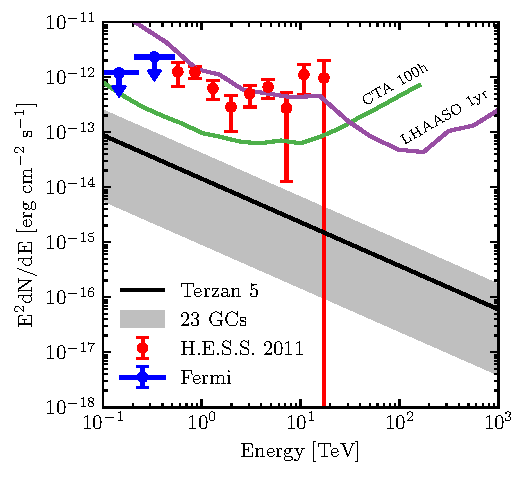
\includegraphics{Figures/Globular/TeV.pdf}
    \caption{Extrapolated spectra for Terzan 5 (black line) and 23 GCs with the IC component detected (grey region). The H.E.S.S. measurement of Terzan 5 is shown by red dots with error bars. The {\it Fermi}-LAT only find upper limits (blue arrows) for Terzan 5 in this energy range. Also included are the sensitivities for 100-hour CTA South (green line) and 1-year LHAASO (purple line).}
    \label{fig:TeV}
\end{figure}

\section{Summary and Conclusions}\label{sec:conclusion}

We have reanalyzed \textit{Fermi}-LAT data in the energy range between 300 MeV and 500 GeV from the direction of 157 GCs in the~\citet{1996AJ....112.1487H} catalog. Using the same data cuts adopted in the construction of the 4FGL catalog, we confirmed the detection of 30 GCs in $\gamma$ rays, and updated the $\gamma$-ray spectral parameters for the sample of detected objects. We also estimated the 95\% C.L. luminosity upper limits for the sample of 127 undetected GCs in the 4FGL catalog. The main objective of our reanalysis was to find evidence for IC emission from $e^{\pm}$ injected by MSPs in GCs. This was done using two different methodologies. First, we searched for correlations of the $\gamma$-ray luminosities with other GCs properties. Second, we performed a spectral analysis of the GCs with a universal fit method that enhances the sensitivity to the high energy tail of the spectra. Specifically:

\begin{itemize}
    \item[1.] Using an expectation-maximization algorithm that properly incorporates null detections ($L_\gamma$ upper limits) in the pipeline, we found a correlation between $L_\gamma$ and the GCs' total photon field energy density $u_\mathrm{Total}$ of the form, \begin{equation}
    \log\left(\frac{L_\gamma}{\mathrm{erg}\;\mathrm{s}^{-1}}\right) = (0.59 \pm 0.09)\log\left(\frac{u_\mathrm{Total}}{\mathrm{eV}\;\mathrm{cm}^{-3}}\right) + (32.97 \pm 0.19).
    \end{equation}
    Using the Kendall $\tau$ coefficient as the test statistic we determined this correlation to have a $3.8\sigma$ significance. The total photon field is dominated by the stellar light of the GCs  ($u_{\rm GC}$), and we find a much weaker correlation (below the 2$\sigma$ level) when only the photon field at the location of the GC ($u_{\rm MW}$) is used. In addition, we obtained a strong correlation (at 6.4$\sigma$ significance) between $L_\gamma$ and the stellar encounter rate $\Gamma_c$, which is given by 
    \begin{equation}
    \log\left(\frac{L_\gamma}{\mathrm{erg}\;\mathrm{s}^{-1}}\right) = (0.39 \pm 0.10)\log\left(\Gamma_c\right) + (32.99 \pm 0.26).
    \end{equation}
    Finally, we found only weak evidence (below the 2$\sigma$ level) for a correlations between $L_\gamma$ and the stellar metallicity [Fe/H].
    \item[2.] We revealed a hidden correlation between $u_\mathrm{Total}$ and $\Gamma_c$, which implies that the $L_\gamma$--$u_{\rm Total}$ and $L_\gamma$--$\Gamma_c$ correlations are not entirely independent. However, as described below, we find spectral evidence for IC emission. The correlation results are consistent with there being both a significant role for dynamical formation of MSPs in GCs and the for the presence of a significant contribution of IC to the observed $\gamma$-ray luminosity.
    \item[3.] We applied a universal spectral fit to the sample of 30 GCs in the 4FGL catalog and searched for evidence of an IC component on top of a curvature radiation model--accounting for the MSPs prompt emission in the GCs. We found that the extra power-law IC component is preferred at the 8.2$\sigma$ significance over the curvature radiation model only. The best-fit power law index of the IC component was found to be $2.79 \pm 0.25$. This implies a power-law $e^\pm$ spectrum with an index of $4.58 \pm 0.50$ and a minimum energy as low as $\sim$ 10 GeV. 
    \item[4.] We estimated the $e^\pm$ injection efficiency $f_{e^\pm}$ for MSPs residing in GCs. We determined the IC $\gamma$-ray luminosities over 300 MeV to 500 GeV, which roughly corresponds to $e^\pm$ energies from 10 GeV to 1 TeV. We found the fraction of MSP spin-down energy injected to $e^\pm$ is comparable to or slightly smaller than that injected to $\gamma$ rays, $f_{e^\pm} \lesssim f_\gamma$ and is at $\lesssim 10\%$ level. This parameter has been estimated in different environments, such as {nearby pulsars~\citep{2017PhRvD..96j3013H, 2018PhRvD..98d3005H, 2021arXiv210400014H}}, the Galactic center~\citep{2013MNRAS.435L..14B}, individual GCs~\citep{2019MNRAS.484.2876M}, and galaxies with low specific star formation rate~\citep{2020arXiv200508982S}. Our results provide new insights into the $f_{e^\pm}$ parameter based on the universal properties of $\gamma$-ray-detected GCs in the Milky Way.
\end{itemize}

In summary, our analysis reveals strong evidence for {soft} IC emission in \textit{Fermi}-LAT GCs. This is indicative of $e^\pm$ injected by MSPs hosted by such systems. Although the {\it Fermi}-LAT sensitivity for energies larger than 10 GeV is not sufficiently high to claim a detection in each individual GC, we employed a universal fit method with the bin-by-bin spectra of the sample of detected objects and were able to increase the sensitivity to the IC component. Our results also explain why it is difficult to detect GCs with TeV $\gamma$-ray telescopes: we have obtained a very soft spectra for the high energy tail of the GC population. It is possible that with a more aggressive observation campaign such objects could be detected by forthcoming TeV telescopes [see~\citep{2018MNRAS.473..897N} for a recent sensitivity analysis] such as CTA~\citep{2019scta.book.....C} and LHAASO~\citep{2019arXiv190502773B}. Globular clusters remain some of the most important systems within which to search for and study millisecond pulsars. We have shown the potential of extracting critical knowledge from $\gamma$-ray data of globular clusters with advanced statistical tools and intensive modelling. 

\chapter{Discussion} \label{ch:discussion}
\chapter{Conclusions} \label{ch:conclusions}
\chapter{Summary} \label{ch:summary}

% This is the standard bibtex file. Do not include the .bib extension in <bib_file_name>.
% Uncomment the following lines to include your bibliography: 
\bibliography{VTthesis}
\bibliographystyle{plainnat}   

% This formats the chapter name to appendix to properly define the headers:
\appendix

% Add your appendices here. You must leave the appendices enclosed in the appendices environment in order for the table of contents to be correct.
\begin{appendices}
  \chapter{First Appendix} \label{app:appendix_one}
  \section{Section one} \label{ase:app_one_sect_1}
  \lipsum[1-3]
  \section{Section two} \label{ase:app_one_sect_2}
  \lipsum[1-3]
  \chapter{Second Appendix} \label{app:appendix_two}
  \lipsum[2]
\end{appendices}

\end{document}

%****************************************************************************
% Below are some general suggestions for writing your dissertation:
%
% 1. Label everything with a meaningful prefix so that you
%    can refer back to sections, tables, figures, equations, etc.
%    Usage \label{<prefix>:<label_name>} where some suggested
%    prefixes are:
%			ch: Chapter
%     		se: Section
%     		ss: Subsection
%     		sss: Sub-subsection
%			app: Appendix
%     		ase: Appendix section
%     		tab: Tables
%     		fig: Figures
%     		sfig: Sub-figures
%     		eq: Equations
%
% 2. The VTthesis class provides for natbib citations. You should upload
%	 one or more *.bib bibtex files. Suppose you have two bib files: some_refs.bib and 
%    other_refs.bib.  Then your bibliography line to include them
%    will be:
%      \bibliography{some_refs, other_refs}
%    where multiple files are separated by commas. In the body of 
%    your work, you can cite your references using natbib citations.
%    Examples:
%      Citation                     Output
%      -------------------------------------------------------
%      \cite{doe_title_2016}        [18]
%      \citet{doe_title_2016}       Doe et al. [18]
%      \citet*{doe_title_2016}      Doe, Jones, and Smith [18]
%
%    For a complete list of options, see
%      https://www.ctan.org/pkg/natbib?lang=en
%
% 3. Here is a sample table. Notice that the caption is centered at the top. Also
%    notice that we use booktabs formatting. You should not use vertical lines
%    in your tables.
% 
%				\begin{table}[htb]
%					\centering
%					\caption{Approximate computation times in hh:mm:ss for full order versus reduced order models.}
%					\begin{tabular}{ccc}
%						\toprule
%						& \multicolumn{2}{c}{Computation Time}\\
%						\cmidrule(r){2-3}
%						$\overline{U}_{in}$ m/s & Full Model & ROM \\
%						\midrule
%						0.90 & 2:00:00 & 2:08:00\\
%						0.88 & 2:00:00 & 0:00:03\\
%						0.92 & 2:00:00 & 0:00:03\\
%						\midrule
%						Total & 6:00:00 & 2:08:06\\
%						\bottomrule
%					\end{tabular}
%					\label{tab:time_rom}
%				\end{table}
% 
% 4. Below are some sample figures. Notice the caption is centered below the
%    figure.
%    a. Single centered figure:
%					\begin{figure}[htb]
%						\centering
%						\includegraphics[scale=0.5]{my_figure.eps}
%						\caption{Average outlet velocity magnitude given an average  
%				        input velocity magnitude of 0.88 m/s.} 
%						\label{fig:output_rom}
%					\end{figure}
%    b. Two by two grid of figures with subcaptions
%					\begin{figure}[htb]
%						\centering
%						\begin{subfigure}[h]{0.45\textwidth}
%							\centering
%							\includegraphics[scale=0.4]{figure_1_1.eps}
%							\caption{Subcaption number one}
%							\label{sfig:first_subfig}
%						\end{subfigure}
%						\begin{subfigure}[h]{0.45\textwidth}
%							\centering
%							\includegraphics[scale=0.4]{figure_1_2.png}
%							\caption{Subcaption number two}
%							\label{sfig:second_subfig}
%						\end{subfigure}
%
%						\begin{subfigure}[h]{0.45\textwidth}
%							\centering
%							\includegraphics[scale=0.4]{figure_2_1.pdf}
%							\caption{Subcaption number three}
%							\label{sfig:third_subfig}
%						\end{subfigure}
%						\begin{subfigure}[h]{0.45\textwidth}
%							\centering
%							\includegraphics[scale=0.4]{figure_2_2.eps}
%							\caption{Subcaption number four}
%							\label{sfig:fourth_subfig}
%						\end{subfigure}
%						\caption{Here is my main caption describing the relationship between the 4 subimages}
%						\label{fig:main_figure}
%					\end{figure}
%
%----------------------------------------------------------------------------
%
% The following is a list of definitions and packages provided by VTthesis:
%
% A. The following packages are provided by the VTthesis class:
%      amsmath, amsthm, amssymb, enumerate, natbib, hyperref, graphicx, 
%      tikz (with shapes and arrows libraries), caption, subcaption,
%      listings, verbatim
%
% B. The following theorem environments are defined by VTthesis:
%      theorem, proposition, lemma, corollary, conjecture
% 
% C. The following definition environments are defined by VTthesis:
%      definition, example, remark, algorithm
%
%----------------------------------------------------------------------------
%
%  I hope this template file and the VTthesis class will keep you from having 
%  to worry about the formatting and allow you to focus on the actual writing.
%  Good luck, and happy writing.
%    Alan Lattimer, VT, 2016
%
%****************************************************************************